

\documentclass[useAMS,usenatbib]{mn2e}

% The usenatbib command allows the use of Patrick Daly's natbib.sty for
% cross-referencing.
%
% If you wish to typeset the paper in Times font (if you do not have the
% PostScript Type 1 Computer Modern fonts you will need to do this to get
% smoother fonts in a PDF file) then uncomment the next line
% \usepackage{Times}

%%%%% AUTHORS - PLACE YOUR OWN MACROS HERE %%%%%
%  These Macros are taken from the AAS TeX macro package version 4.0.
%  Include this file in your LaTeX source only if you are not using
%  the AAS TeX macro package and need to resolve the macro definitions
%  in the BibTeX entries returned by the ADS abstract service.
%
%  If you plan not to use this file to resolve the journal macros
%  rather than the whole AAS TeX macro package, you should save the
%  file as ``aas_macros.sty'' and then include it in your paper by
%  using a construct such as:
%\documentstyle[11pt,aas_macros]{article}
%
%  For more information on the AASTeX macro package, please see the URL
%http://www.aas.org/publications/aastex.html
%  For more information about ADS abstract server, please see the URL
%http://adswww.harvard.edu/ads_abstracts.html
%

% Abbreviations for journals.  The object here is to provide authors
% with convenient shorthands for the most ``popular'' (often-cited)
% journals; the author can use these markup tags without being concerned
% about the exact form of the journal abbreviation, or its formatting.
% It is up to the keeper of the macros to make sure the macros expand
% to the proper text.  If macro package writers agree to all use the
% same TeX command name, authors only have to remember one thing, and
% the style file will take care of editorial preferences.  This also
% applies when a single journal decides to revamp its abbreviating
% scheme, as happened with the ApJ (Abt 1991).

\let\jnlstyle=\rm
\def\refjnl#1{{\jnlstyle#1}}

\def\aj{\refjnl{AJ}}                   % Astronomical Journal
\def\araa{\refjnl{ARA\&A}}             % Annual Review of Astron and Astrophys
\def\apj{\refjnl{ApJ}}                 % Astrophysical Journal
\def\apjl{\refjnl{ApJ}}                % Astrophysical Journal, Letters
\def\apjs{\refjnl{ApJS}}               % Astrophysical Journal, Supplement
\def\ao{\refjnl{Appl.~Opt.}}           % Applied Optics
\def\apss{\refjnl{Ap\&SS}}             % Astrophysics and Space Science
\def\aap{\refjnl{A\&A}}                % Astronomy and Astrophysics
\def\aapr{\refjnl{A\&A~Rev.}}          % Astronomy and Astrophysics Reviews
\def\aaps{\refjnl{A\&AS}}              % Astronomy and Astrophysics, Supplement
\def\azh{\refjnl{AZh}}                 % Astronomicheskii Zhurnal
\def\baas{\refjnl{BAAS}}               % Bulletin of the AAS
\def\jrasc{\refjnl{JRASC}}             % Journal of the RAS of Canada
\def\memras{\refjnl{MmRAS}}            % Memoirs of the RAS
\def\mnras{\refjnl{MNRAS}}             % Monthly Notices of the RAS
\def\pra{\refjnl{Phys.~Rev.~A}}        % Physical Review A: General Physics
\def\prb{\refjnl{Phys.~Rev.~B}}        % Physical Review B: Solid State
\def\prc{\refjnl{Phys.~Rev.~C}}        % Physical Review C
\def\prd{\refjnl{Phys.~Rev.~D}}        % Physical Review D
\def\pre{\refjnl{Phys.~Rev.~E}}        % Physical Review E
\def\prl{\refjnl{Phys.~Rev.~Lett.}}    % Physical Review Letters
\def\pasp{\refjnl{PASP}}               % Publications of the ASP
\def\pasj{\refjnl{PASJ}}               % Publications of the ASJ
\def\qjras{\refjnl{QJRAS}}             % Quarterly Journal of the RAS
\def\skytel{\refjnl{S\&T}}             % Sky and Telescope
\def\solphys{\refjnl{Sol.~Phys.}}      % Solar Physics
\def\sovast{\refjnl{Soviet~Ast.}}      % Soviet Astronomy
\def\ssr{\refjnl{Space~Sci.~Rev.}}     % Space Science Reviews
\def\zap{\refjnl{ZAp}}                 % Zeitschrift fuer Astrophysik
\def\nat{\refjnl{Nature}}              % Nature
\def\iaucirc{\refjnl{IAU~Circ.}}       % IAU Cirulars
\def\aplett{\refjnl{Astrophys.~Lett.}} % Astrophysics Letters
\def\apspr{\refjnl{Astrophys.~Space~Phys.~Res.}}
                % Astrophysics Space Physics Research
\def\bain{\refjnl{Bull.~Astron.~Inst.~Netherlands}} 
                % Bulletin Astronomical Institute of the Netherlands
\def\fcp{\refjnl{Fund.~Cosmic~Phys.}}  % Fundamental Cosmic Physics
\def\gca{\refjnl{Geochim.~Cosmochim.~Acta}}   % Geochimica Cosmochimica Acta
\def\grl{\refjnl{Geophys.~Res.~Lett.}} % Geophysics Research Letters
\def\jcp{\refjnl{J.~Chem.~Phys.}}      % Journal of Chemical Physics
\def\jgr{\refjnl{J.~Geophys.~Res.}}    % Journal of Geophysics Research
\def\jqsrt{\refjnl{J.~Quant.~Spec.~Radiat.~Transf.}}
                % Journal of Quantitiative Spectroscopy and Radiative Transfer
\def\memsai{\refjnl{Mem.~Soc.~Astron.~Italiana}}
                % Mem. Societa Astronomica Italiana
\def\nphysa{\refjnl{Nucl.~Phys.~A}}   % Nuclear Physics A
\def\physrep{\refjnl{Phys.~Rep.}}   % Physics Reports
\def\physscr{\refjnl{Phys.~Scr}}   % Physica Scripta
\def\planss{\refjnl{Planet.~Space~Sci.}}   % Planetary Space Science
\def\procspie{\refjnl{Proc.~SPIE}}   % Proceedings of the SPIE

\let\astap=\aap
\let\apjlett=\apjl
\let\apjsupp=\apjs
\let\applopt=\ao


% Psfig/TeX 
\def\PsfigVersion{1.9}
% dvips version
%
% All psfig/tex software, documentation, and related files
% in this distribution of psfig/tex are 
% Copyright 1987, 1988, 1991 Trevor J. Darrell
%
% Permission is granted for use and non-profit distribution of psfig/tex 
% providing that this notice is clearly maintained. The right to
% distribute any portion of psfig/tex for profit or as part of any commercial
% product is specifically reserved for the author(s) of that portion.
%
% *** Feel free to make local modifications of psfig as you wish,
% *** but DO NOT post any changed or modified versions of ``psfig''
% *** directly to the net. Send them to me and I'll try to incorporate
% *** them into future versions. If you want to take the psfig code 
% *** and make a new program (subject to the copyright above), distribute it, 
% *** (and maintain it) that's fine, just don't call it psfig.
%
% Bugs and improvements to trevor@media.mit.edu.
%
% Thanks to Greg Hager (GDH) and Ned Batchelder for their contributions
% to the original version of this project.
%
% Modified by J. Daniel Smith on 9 October 1990 to accept the
% %%BoundingBox: comment with or without a space after the colon.  Stole
% file reading code from Tom Rokicki's EPSF.TEX file (see below).
%
% More modifications by J. Daniel Smith on 29 March 1991 to allow the
% the included PostScript figure to be rotated.  The amount of
% rotation is specified by the "angle=" parameter of the \psfig command.
%
% Modified by Robert Russell on June 25, 1991 to allow users to specify
% .ps filenames which don't yet exist, provided they explicitly provide
% boundingbox information via the \psfig command. Note: This will only work
% if the "file=" parameter follows all four "bb???=" parameters in the
% command. This is due to the order in which psfig interprets these params.
%
%  3 Jul 1991	JDS	check if file already read in once
%  4 Sep 1991	JDS	fixed incorrect computation of rotated
%			bounding box
% 25 Sep 1991	GVR	expanded synopsis of \psfig
% 14 Oct 1991	JDS	\fbox code from LaTeX so \psdraft works with TeX
%			changed \typeout to \ps@typeout
% 17 Oct 1991	JDS	added \psscalefirst and \psrotatefirst
%

% From: gvr@cs.brown.edu (George V. Reilly)
%
% \psdraft	draws an outline box, but doesn't include the figure
%		in the DVI file.  Useful for previewing.
%
% \psfull	includes the figure in the DVI file (default).
%
% \psscalefirst width= or height= specifies the size of the figure
% 		before rotation.
% \psrotatefirst (default) width= or height= specifies the size of the
% 		 figure after rotation.  Asymetric figures will
% 		 appear to shrink.
%
% \psfigurepath#1	sets the path to search for the figure
%
% \psfig
% usage: \psfig{file=, figure=, height=, width=,
%			bbllx=, bblly=, bburx=, bbury=,
%			rheight=, rwidth=, clip=, angle=, silent=}
%
%	"file" is the filename.  If no path name is specified and the
%		file is not found in the current directory,
%		it will be looked for in directory \psfigurepath.
%	"figure" is a synonym for "file".
%	By default, the width and height of the figure are taken from
%		the BoundingBox of the figure.
%	If "width" is specified, the figure is scaled so that it has
%		the specified width.  Its height changes proportionately.
%	If "height" is specified, the figure is scaled so that it has
%		the specified height.  Its width changes proportionately.
%	If both "width" and "height" are specified, the figure is scaled
%		anamorphically.
%	"bbllx", "bblly", "bburx", and "bbury" control the PostScript
%		BoundingBox.  If these four values are specified
%               *before* the "file" option, the PSFIG will not try to
%               open the PostScript file.
%	"rheight" and "rwidth" are the reserved height and width
%		of the figure, i.e., how big TeX actually thinks
%		the figure is.  They default to "width" and "height".
%	The "clip" option ensures that no portion of the figure will
%		appear outside its BoundingBox.  "clip=" is a switch and
%		takes no value, but the `=' must be present.
%	The "angle" option specifies the angle of rotation (degrees, ccw).
%	The "silent" option makes \psfig work silently.
%

% check to see if macros already loaded in (maybe some other file says
% "\input psfig") ...
\ifx\undefined\psfig\else\endinput\fi

%
% from a suggestion by eijkhout@csrd.uiuc.edu to allow
% loading as a style file. Changed to avoid problems
% with amstex per suggestion by jbence@math.ucla.edu

\let\LaTeXAtSign=\@
\let\@=\relax
\edef\psfigRestoreAt{\catcode`\@=\number\catcode`@\relax}
%\edef\psfigRestoreAt{\catcode`@=\number\catcode`@\relax}
\catcode`\@=11\relax
\newwrite\@unused
\def\ps@typeout#1{{\let\protect\string\immediate\write\@unused{#1}}}
%\ps@typeout{psfig/tex \PsfigVersion}

%% Here's how you define your figure path.  Should be set up with null
%% default and a user useable definition.

\def\figurepath{./}
\def\psfigurepath#1{\edef\figurepath{#1}}

%
% @psdo control structure -- similar to Latex @for.
% I redefined these with different names so that psfig can
% be used with TeX as well as LaTeX, and so that it will not 
% be vunerable to future changes in LaTeX's internal
% control structure,
%
\def\@nnil{\@nil}
\def\@empty{}
\def\@psdonoop#1\@@#2#3{}
\def\@psdo#1:=#2\do#3{\edef\@psdotmp{#2}\ifx\@psdotmp\@empty \else
    \expandafter\@psdoloop#2,\@nil,\@nil\@@#1{#3}\fi}
\def\@psdoloop#1,#2,#3\@@#4#5{\def#4{#1}\ifx #4\@nnil \else
       #5\def#4{#2}\ifx #4\@nnil \else#5\@ipsdoloop #3\@@#4{#5}\fi\fi}
\def\@ipsdoloop#1,#2\@@#3#4{\def#3{#1}\ifx #3\@nnil 
       \let\@nextwhile=\@psdonoop \else
      #4\relax\let\@nextwhile=\@ipsdoloop\fi\@nextwhile#2\@@#3{#4}}
\def\@tpsdo#1:=#2\do#3{\xdef\@psdotmp{#2}\ifx\@psdotmp\@empty \else
    \@tpsdoloop#2\@nil\@nil\@@#1{#3}\fi}
\def\@tpsdoloop#1#2\@@#3#4{\def#3{#1}\ifx #3\@nnil 
       \let\@nextwhile=\@psdonoop \else
      #4\relax\let\@nextwhile=\@tpsdoloop\fi\@nextwhile#2\@@#3{#4}}
% 
% \fbox is defined in latex.tex; so if \fbox is undefined, assume that
% we are not in LaTeX.
% Perhaps this could be done better???
\ifx\undefined\fbox
% \fbox code from modified slightly from LaTeX
\newdimen\fboxrule
\newdimen\fboxsep
\newdimen\ps@tempdima
\newbox\ps@tempboxa
\fboxsep = 3pt
\fboxrule = .4pt
\long\def\fbox#1{\leavevmode\setbox\ps@tempboxa\hbox{#1}\ps@tempdima\fboxrule
    \advance\ps@tempdima \fboxsep \advance\ps@tempdima \dp\ps@tempboxa
   \hbox{\lower \ps@tempdima\hbox
  {\vbox{\hrule height \fboxrule
          \hbox{\vrule width \fboxrule \hskip\fboxsep
          \vbox{\vskip\fboxsep \box\ps@tempboxa\vskip\fboxsep}\hskip 
                 \fboxsep\vrule width \fboxrule}
                 \hrule height \fboxrule}}}}
\fi
%
%%%%%%%%%%%%%%%%%%%%%%%%%%%%%%%%%%%%%%%%%%%%%%%%%%%%%%%%%%%%%%%%%%%
% file reading stuff from epsf.tex
%   EPSF.TEX macro file:
%   Written by Tomas Rokicki of Radical Eye Software, 29 Mar 1989.
%   Revised by Don Knuth, 3 Jan 1990.
%   Revised by Tomas Rokicki to accept bounding boxes with no
%      space after the colon, 18 Jul 1990.
%   Portions modified/removed for use in PSFIG package by
%      J. Daniel Smith, 9 October 1990.
%
\newread\ps@stream
\newif\ifnot@eof       % continue looking for the bounding box?
\newif\if@noisy        % report what you're making?
\newif\if@atend        % %%BoundingBox: has (at end) specification
\newif\if@psfile       % does this look like a PostScript file?
%
% PostScript files should start with `%!'
%
{\catcode`\%=12\global\gdef\epsf@start{%!}}
\def\epsf@PS{PS}
%
\def\epsf@getbb#1{%
%
%   The first thing we need to do is to open the
%   PostScript file, if possible.
%
\openin\ps@stream=#1
\ifeof\ps@stream\ps@typeout{Error, File #1 not found}\else
%
%   Okay, we got it. Now we'll scan lines until we find one that doesn't
%   start with %. We're looking for the bounding box comment.
%
   {\not@eoftrue \chardef\other=12
    \def\do##1{\catcode`##1=\other}\dospecials \catcode`\ =10
    \loop
       \if@psfile
	  \read\ps@stream to \epsf@fileline
       \else{
	  \obeyspaces
          \read\ps@stream to \epsf@tmp\global\let\epsf@fileline\epsf@tmp}
       \fi
       \ifeof\ps@stream\not@eoffalse\else
%
%   Check the first line for `%!'.  Issue a warning message if its not
%   there, since the file might not be a PostScript file.
%
       \if@psfile\else
       \expandafter\epsf@test\epsf@fileline:. \\%
       \fi
%
%   We check to see if the first character is a % sign;
%   if so, we look further and stop only if the line begins with
%   `%%BoundingBox:' and the `(atend)' specification was not found.
%   That is, the only way to stop is when the end of file is reached,
%   or a `%%BoundingBox: llx lly urx ury' line is found.
%
          \expandafter\epsf@aux\epsf@fileline:. \\%
       \fi
   \ifnot@eof\repeat
   }\closein\ps@stream\fi}%
%
% This tests if the file we are reading looks like a PostScript file.
%
\long\def\epsf@test#1#2#3:#4\\{\def\epsf@testit{#1#2}
			\ifx\epsf@testit\epsf@start\else
\ps@typeout{Warning! File does not start with `\epsf@start'.  It may not be a PostScript file.}
			\fi
			\@psfiletrue} % don't test after 1st line
%
%   We still need to define the tricky \epsf@aux macro. This requires
%   a couple of magic constants for comparison purposes.
%
{\catcode`\%=12\global\let\epsf@percent=%\global\def\epsf@bblit{%BoundingBox}}
%
%
%   So we're ready to check for `%BoundingBox:' and to grab the
%   values if they are found.  We continue searching if `(at end)'
%   was found after the `%BoundingBox:'.
%
\long\def\epsf@aux#1#2:#3\\{\ifx#1\epsf@percent
   \def\epsf@testit{#2}\ifx\epsf@testit\epsf@bblit
	\@atendfalse
        \epsf@atend #3 . \\%
	\if@atend	
	   \if@verbose{
		\ps@typeout{psfig: found `(atend)'; continuing search}
	   }\fi
        \else
        \epsf@grab #3 . . . \\%
        \not@eoffalse
        \global\no@bbfalse
        \fi
   \fi\fi}%
%
%   Here we grab the values and stuff them in the appropriate definitions.
%
\def\epsf@grab #1 #2 #3 #4 #5\\{%
   \global\def\epsf@llx{#1}\ifx\epsf@llx\empty
      \epsf@grab #2 #3 #4 #5 .\\\else
   \global\def\epsf@lly{#2}%
   \global\def\epsf@urx{#3}\global\def\epsf@ury{#4}\fi}%
%
% Determine if the stuff following the %%BoundingBox is `(atend)'
% J. Daniel Smith.  Copied from \epsf@grab above.
%
\def\epsf@atendlit{(atend)} 
\def\epsf@atend #1 #2 #3\\{%
   \def\epsf@tmp{#1}\ifx\epsf@tmp\empty
      \epsf@atend #2 #3 .\\\else
   \ifx\epsf@tmp\epsf@atendlit\@atendtrue\fi\fi}


% End of file reading stuff from epsf.tex
%%%%%%%%%%%%%%%%%%%%%%%%%%%%%%%%%%%%%%%%%%%%%%%%%%%%%%%%%%%%%%%%%%%

%%%%%%%%%%%%%%%%%%%%%%%%%%%%%%%%%%%%%%%%%%%%%%%%%%%%%%%%%%%%%%%%%%%
% trigonometry stuff from "trig.tex"
\chardef\psletter = 11 % won't conflict with \begin{letter} now...
\chardef\other = 12

\newif \ifdebug %%% turn me on to see TeX hard at work ...
\newif\ifc@mpute %%% don't need to compute some values
\c@mputetrue % but assume that we do

\let\then = \relax
\def\r@dian{pt }
\let\r@dians = \r@dian
\let\dimensionless@nit = \r@dian
\let\dimensionless@nits = \dimensionless@nit
\def\internal@nit{sp }
\let\internal@nits = \internal@nit
\newif\ifstillc@nverging
\def \Mess@ge #1{\ifdebug \then \message {#1} \fi}

{ %%% Things that need abnormal catcodes %%%
	\catcode `\@ = \psletter
	\gdef \nodimen {\expandafter \n@dimen \the \dimen}
	\gdef \term #1 #2 #3%
	       {\edef \t@ {\the #1}%%% freeze parameter 1 (count, by value)
		\edef \t@@ {\expandafter \n@dimen \the #2\r@dian}%
				   %%% freeze parameter 2 (dimen, by value)
		\t@rm {\t@} {\t@@} {#3}%
	       }
	\gdef \t@rm #1 #2 #3%
	       {{%
		\count 0 = 0
		\dimen 0 = 1 \dimensionless@nit
		\dimen 2 = #2\relax
		\Mess@ge {Calculating term #1 of \nodimen 2}%
		\loop
		\ifnum	\count 0 < #1
		\then	\advance \count 0 by 1
			\Mess@ge {Iteration \the \count 0 \space}%
			\Multiply \dimen 0 by {\dimen 2}%
			\Mess@ge {After multiplication, term = \nodimen 0}%
			\Divide \dimen 0 by {\count 0}%
			\Mess@ge {After division, term = \nodimen 0}%
		\repeat
		\Mess@ge {Final value for term #1 of 
				\nodimen 2 \space is \nodimen 0}%
		\xdef \Term {#3 = \nodimen 0 \r@dians}%
		\aftergroup \Term
	       }}
	\catcode `\p = \other
	\catcode `\t = \other
	\gdef \n@dimen #1pt{#1} %%% throw away the ``pt''
}

\def \Divide #1by #2{\divide #1 by #2} %%% just a synonym

\def \Multiply #1by #2%%% allows division of a dimen by a dimen
       {{%%% should really freeze parameter 2 (dimen, passed by value)
	\count 0 = #1\relax
	\count 2 = #2\relax
	\count 4 = 65536
	\Mess@ge {Before scaling, count 0 = \the \count 0 \space and
			count 2 = \the \count 2}%
	\ifnum	\count 0 > 32767 %%% do our best to avoid overflow
	\then	\divide \count 0 by 4
		\divide \count 4 by 4
	\else	\ifnum	\count 0 < -32767
		\then	\divide \count 0 by 4
			\divide \count 4 by 4
		\else
		\fi
	\fi
	\ifnum	\count 2 > 32767 %%% while retaining reasonable accuracy
	\then	\divide \count 2 by 4
		\divide \count 4 by 4
	\else	\ifnum	\count 2 < -32767
		\then	\divide \count 2 by 4
			\divide \count 4 by 4
		\else
		\fi
	\fi
	\multiply \count 0 by \count 2
	\divide \count 0 by \count 4
	\xdef \product {#1 = \the \count 0 \internal@nits}%
	\aftergroup \product
       }}

\def\r@duce{\ifdim\dimen0 > 90\r@dian \then   % sin(x+90) = sin(180-x)
		\multiply\dimen0 by -1
		\advance\dimen0 by 180\r@dian
		\r@duce
	    \else \ifdim\dimen0 < -90\r@dian \then  % sin(-x) = sin(360+x)
		\advance\dimen0 by 360\r@dian
		\r@duce
		\fi
	    \fi}

\def\Sine#1%
       {{%
	\dimen 0 = #1 \r@dian
	\r@duce
	\ifdim\dimen0 = -90\r@dian \then
	   \dimen4 = -1\r@dian
	   \c@mputefalse
	\fi
	\ifdim\dimen0 = 90\r@dian \then
	   \dimen4 = 1\r@dian
	   \c@mputefalse
	\fi
	\ifdim\dimen0 = 0\r@dian \then
	   \dimen4 = 0\r@dian
	   \c@mputefalse
	\fi
%
	\ifc@mpute \then
        	% convert degrees to radians
		\divide\dimen0 by 180
		\dimen0=3.141592654\dimen0
%
		\dimen 2 = 3.1415926535897963\r@dian %%% a well-known constant
		\divide\dimen 2 by 2 %%% we only deal with -pi/2 : pi/2
		\Mess@ge {Sin: calculating Sin of \nodimen 0}%
		\count 0 = 1 %%% see power-series expansion for sine
		\dimen 2 = 1 \r@dian %%% ditto
		\dimen 4 = 0 \r@dian %%% ditto
		\loop
			\ifnum	\dimen 2 = 0 %%% then we've done
			\then	\stillc@nvergingfalse 
			\else	\stillc@nvergingtrue
			\fi
			\ifstillc@nverging %%% then calculate next term
			\then	\term {\count 0} {\dimen 0} {\dimen 2}%
				\advance \count 0 by 2
				\count 2 = \count 0
				\divide \count 2 by 2
				\ifodd	\count 2 %%% signs alternate
				\then	\advance \dimen 4 by \dimen 2
				\else	\advance \dimen 4 by -\dimen 2
				\fi
		\repeat
	\fi		
			\xdef \sine {\nodimen 4}%
       }}

% Now the Cosine can be calculated easily by calling \Sine
\def\Cosine#1{\ifx\sine\UnDefined\edef\Savesine{\relax}\else
		             \edef\Savesine{\sine}\fi
	{\dimen0=#1\r@dian\advance\dimen0 by 90\r@dian
	 \Sine{\nodimen 0}
	 \xdef\cosine{\sine}
	 \xdef\sine{\Savesine}}}	      
% end of trig stuff
%%%%%%%%%%%%%%%%%%%%%%%%%%%%%%%%%%%%%%%%%%%%%%%%%%%%%%%%%%%%%%%%%%%%

\def\psdraft{
	\def\@psdraft{0}
	%\ps@typeout{draft level now is \@psdraft \space . }
}
\def\psfull{
	\def\@psdraft{100}
	%\ps@typeout{draft level now is \@psdraft \space . }
}

\psfull

\newif\if@scalefirst
\def\psscalefirst{\@scalefirsttrue}
\def\psrotatefirst{\@scalefirstfalse}
\psrotatefirst

\newif\if@draftbox
\def\psnodraftbox{
	\@draftboxfalse
}
\def\psdraftbox{
	\@draftboxtrue
}
\@draftboxtrue

\newif\if@prologfile
\newif\if@postlogfile
\def\pssilent{
	\@noisyfalse
}
\def\psnoisy{
	\@noisytrue
}
\psnoisy
%%% These are for the option list.
%%% A specification of the form a = b maps to calling \@p@@sa{b}
\newif\if@bbllx
\newif\if@bblly
\newif\if@bburx
\newif\if@bbury
\newif\if@height
\newif\if@width
\newif\if@rheight
\newif\if@rwidth
\newif\if@angle
\newif\if@clip
\newif\if@verbose
\def\@p@@sclip#1{\@cliptrue}


\newif\if@decmpr

%%% GDH 7/26/87 -- changed so that it first looks in the local directory,
%%% then in a specified global directory for the ps file.
%%% RPR 6/25/91 -- changed so that it defaults to user-supplied name if
%%% boundingbox info is specified, assuming graphic will be created by
%%% print time.
%%% TJD 10/19/91 -- added bbfile vs. file distinction, and @decmpr flag

\def\@p@@sfigure#1{\def\@p@sfile{null}\def\@p@sbbfile{null}
	        \openin1=#1.bb
		\ifeof1\closein1
	        	\openin1=\figurepath#1.bb
			\ifeof1\closein1
			        \openin1=#1
				\ifeof1\closein1%
				       \openin1=\figurepath#1
					\ifeof1
					   \ps@typeout{Error, File #1 not found}
						\if@bbllx\if@bblly
				   		\if@bburx\if@bbury
			      				\def\@p@sfile{#1}%
			      				\def\@p@sbbfile{#1}%
							\@decmprfalse
				  	   	\fi\fi\fi\fi
					\else\closein1
				    		\def\@p@sfile{\figurepath#1}%
				    		\def\@p@sbbfile{\figurepath#1}%
						\@decmprfalse
	                       		\fi%
			 	\else\closein1%
					\def\@p@sfile{#1}
					\def\@p@sbbfile{#1}
					\@decmprfalse
			 	\fi
			\else
				\def\@p@sfile{\figurepath#1}
				\def\@p@sbbfile{\figurepath#1.bb}
				\@decmprtrue
			\fi
		\else
			\def\@p@sfile{#1}
			\def\@p@sbbfile{#1.bb}
			\@decmprtrue
		\fi}

\def\@p@@sfile#1{\@p@@sfigure{#1}}

\def\@p@@sbbllx#1{
		%\ps@typeout{bbllx is #1}
		\@bbllxtrue
		\dimen100=#1
		\edef\@p@sbbllx{\number\dimen100}
}
\def\@p@@sbblly#1{
		%\ps@typeout{bblly is #1}
		\@bbllytrue
		\dimen100=#1
		\edef\@p@sbblly{\number\dimen100}
}
\def\@p@@sbburx#1{
		%\ps@typeout{bburx is #1}
		\@bburxtrue
		\dimen100=#1
		\edef\@p@sbburx{\number\dimen100}
}
\def\@p@@sbbury#1{
		%\ps@typeout{bbury is #1}
		\@bburytrue
		\dimen100=#1
		\edef\@p@sbbury{\number\dimen100}
}
\def\@p@@sheight#1{
		\@heighttrue
		\dimen100=#1
   		\edef\@p@sheight{\number\dimen100}
		%\ps@typeout{Height is \@p@sheight}
}
\def\@p@@swidth#1{
		%\ps@typeout{Width is #1}
		\@widthtrue
		\dimen100=#1
		\edef\@p@swidth{\number\dimen100}
}
\def\@p@@srheight#1{
		%\ps@typeout{Reserved height is #1}
		\@rheighttrue
		\dimen100=#1
		\edef\@p@srheight{\number\dimen100}
}
\def\@p@@srwidth#1{
		%\ps@typeout{Reserved width is #1}
		\@rwidthtrue
		\dimen100=#1
		\edef\@p@srwidth{\number\dimen100}
}
\def\@p@@sangle#1{
		%\ps@typeout{Rotation is #1}
		\@angletrue
%		\dimen100=#1
		\edef\@p@sangle{#1} %\number\dimen100}
}
\def\@p@@ssilent#1{ 
		\@verbosefalse
}
\def\@p@@sprolog#1{\@prologfiletrue\def\@prologfileval{#1}}
\def\@p@@spostlog#1{\@postlogfiletrue\def\@postlogfileval{#1}}
\def\@cs@name#1{\csname #1\endcsname}
\def\@setparms#1=#2,{\@cs@name{@p@@s#1}{#2}}
%
% initialize the defaults (size the size of the figure)
%
\def\ps@init@parms{
		\@bbllxfalse \@bbllyfalse
		\@bburxfalse \@bburyfalse
		\@heightfalse \@widthfalse
		\@rheightfalse \@rwidthfalse
		\def\@p@sbbllx{}\def\@p@sbblly{}
		\def\@p@sbburx{}\def\@p@sbbury{}
		\def\@p@sheight{}\def\@p@swidth{}
		\def\@p@srheight{}\def\@p@srwidth{}
		\def\@p@sangle{0}
		\def\@p@sfile{} \def\@p@sbbfile{}
		\def\@p@scost{10}
		\def\@sc{}
		\@prologfilefalse
		\@postlogfilefalse
		\@clipfalse
		\if@noisy
			\@verbosetrue
		\else
			\@verbosefalse
		\fi
}
%
% Go through the options setting things up.
%
\def\parse@ps@parms#1{
	 	\@psdo\@psfiga:=#1\do
		   {\expandafter\@setparms\@psfiga,}}
%
% Compute bb height and width
%
\newif\ifno@bb
\def\bb@missing{
	\if@verbose{
		\ps@typeout{psfig: searching \@p@sbbfile \space  for bounding box}
	}\fi
	\no@bbtrue
	\epsf@getbb{\@p@sbbfile}
        \ifno@bb \else \bb@cull\epsf@llx\epsf@lly\epsf@urx\epsf@ury\fi
}	
\def\bb@cull#1#2#3#4{
	\dimen100=#1 bp\edef\@p@sbbllx{\number\dimen100}
	\dimen100=#2 bp\edef\@p@sbblly{\number\dimen100}
	\dimen100=#3 bp\edef\@p@sbburx{\number\dimen100}
	\dimen100=#4 bp\edef\@p@sbbury{\number\dimen100}
	\no@bbfalse
}
% rotate point (#1,#2) about (0,0).
% The sine and cosine of the angle are already stored in \sine and
% \cosine.  The result is placed in (\p@intvaluex, \p@intvaluey).
\newdimen\p@intvaluex
\newdimen\p@intvaluey
\def\rotate@#1#2{{\dimen0=#1 sp\dimen1=#2 sp
%            	calculate x' = x \cos\theta - y \sin\theta
		  \global\p@intvaluex=\cosine\dimen0
		  \dimen3=\sine\dimen1
		  \global\advance\p@intvaluex by -\dimen3
% 		calculate y' = x \sin\theta + y \cos\theta
		  \global\p@intvaluey=\sine\dimen0
		  \dimen3=\cosine\dimen1
		  \global\advance\p@intvaluey by \dimen3
		  }}
\def\compute@bb{
		\no@bbfalse
		\if@bbllx \else \no@bbtrue \fi
		\if@bblly \else \no@bbtrue \fi
		\if@bburx \else \no@bbtrue \fi
		\if@bbury \else \no@bbtrue \fi
		\ifno@bb \bb@missing \fi
		\ifno@bb \ps@typeout{FATAL ERROR: no bb supplied or found}
			\no-bb-error
		\fi
		%
%\ps@typeout{BB: \@p@sbbllx, \@p@sbblly, \@p@sbburx, \@p@sbbury} 
%
% store height/width of original (unrotated) bounding box
		\count203=\@p@sbburx
		\count204=\@p@sbbury
		\advance\count203 by -\@p@sbbllx
		\advance\count204 by -\@p@sbblly
		\edef\ps@bbw{\number\count203}
		\edef\ps@bbh{\number\count204}
		%\ps@typeout{ psbbh = \ps@bbh, psbbw = \ps@bbw }
		\if@angle 
			\Sine{\@p@sangle}\Cosine{\@p@sangle}
	        	{\dimen100=\maxdimen\xdef\r@p@sbbllx{\number\dimen100}
					    \xdef\r@p@sbblly{\number\dimen100}
			                    \xdef\r@p@sbburx{-\number\dimen100}
					    \xdef\r@p@sbbury{-\number\dimen100}}
%
% Need to rotate all four points and take the X-Y extremes of the new
% points as the new bounding box.
                        \def\minmaxtest{
			   \ifnum\number\p@intvaluex<\r@p@sbbllx
			      \xdef\r@p@sbbllx{\number\p@intvaluex}\fi
			   \ifnum\number\p@intvaluex>\r@p@sbburx
			      \xdef\r@p@sbburx{\number\p@intvaluex}\fi
			   \ifnum\number\p@intvaluey<\r@p@sbblly
			      \xdef\r@p@sbblly{\number\p@intvaluey}\fi
			   \ifnum\number\p@intvaluey>\r@p@sbbury
			      \xdef\r@p@sbbury{\number\p@intvaluey}\fi
			   }
%			lower left
			\rotate@{\@p@sbbllx}{\@p@sbblly}
			\minmaxtest
%			upper left
			\rotate@{\@p@sbbllx}{\@p@sbbury}
			\minmaxtest
%			lower right
			\rotate@{\@p@sbburx}{\@p@sbblly}
			\minmaxtest
%			upper right
			\rotate@{\@p@sbburx}{\@p@sbbury}
			\minmaxtest
			\edef\@p@sbbllx{\r@p@sbbllx}\edef\@p@sbblly{\r@p@sbblly}
			\edef\@p@sbburx{\r@p@sbburx}\edef\@p@sbbury{\r@p@sbbury}
%\ps@typeout{rotated BB: \r@p@sbbllx, \r@p@sbblly, \r@p@sbburx, \r@p@sbbury}
		\fi
		\count203=\@p@sbburx
		\count204=\@p@sbbury
		\advance\count203 by -\@p@sbbllx
		\advance\count204 by -\@p@sbblly
		\edef\@bbw{\number\count203}
		\edef\@bbh{\number\count204}
		%\ps@typeout{ bbh = \@bbh, bbw = \@bbw }
}
%
% \in@hundreds performs #1 * (#2 / #3) correct to the hundreds,
%	then leaves the result in @result
%
\def\in@hundreds#1#2#3{\count240=#2 \count241=#3
		     \count100=\count240	% 100 is first digit #2/#3
		     \divide\count100 by \count241
		     \count101=\count100
		     \multiply\count101 by \count241
		     \advance\count240 by -\count101
		     \multiply\count240 by 10
		     \count101=\count240	%101 is second digit of #2/#3
		     \divide\count101 by \count241
		     \count102=\count101
		     \multiply\count102 by \count241
		     \advance\count240 by -\count102
		     \multiply\count240 by 10
		     \count102=\count240	% 102 is the third digit
		     \divide\count102 by \count241
		     \count200=#1\count205=0
		     \count201=\count200
			\multiply\count201 by \count100
		 	\advance\count205 by \count201
		     \count201=\count200
			\divide\count201 by 10
			\multiply\count201 by \count101
			\advance\count205 by \count201
			%
		     \count201=\count200
			\divide\count201 by 100
			\multiply\count201 by \count102
			\advance\count205 by \count201
			%
		     \edef\@result{\number\count205}
}
\def\compute@wfromh{
		% computing : width = height * (bbw / bbh)
		\in@hundreds{\@p@sheight}{\@bbw}{\@bbh}
		%\ps@typeout{ \@p@sheight * \@bbw / \@bbh, = \@result }
		\edef\@p@swidth{\@result}
		%\ps@typeout{w from h: width is \@p@swidth}
}
\def\compute@hfromw{
		% computing : height = width * (bbh / bbw)
	        \in@hundreds{\@p@swidth}{\@bbh}{\@bbw}
		%\ps@typeout{ \@p@swidth * \@bbh / \@bbw = \@result }
		\edef\@p@sheight{\@result}
		%\ps@typeout{h from w : height is \@p@sheight}
}
\def\compute@handw{
		\if@height 
			\if@width
			\else
				\compute@wfromh
			\fi
		\else 
			\if@width
				\compute@hfromw
			\else
				\edef\@p@sheight{\@bbh}
				\edef\@p@swidth{\@bbw}
			\fi
		\fi
}
\def\compute@resv{
		\if@rheight \else \edef\@p@srheight{\@p@sheight} \fi
		\if@rwidth \else \edef\@p@srwidth{\@p@swidth} \fi
		%\ps@typeout{rheight = \@p@srheight, rwidth = \@p@srwidth}
}
%		
% Compute any missing values
\def\compute@sizes{
	\compute@bb
	\if@scalefirst\if@angle
% at this point the bounding box has been adjsuted correctly for
% rotation.  PSFIG does all of its scaling using \@bbh and \@bbw.  If
% a width= or height= was specified along with \psscalefirst, then the
% width=/height= value needs to be adjusted to match the new (rotated)
% bounding box size (specifed in \@bbw and \@bbh).
%    \ps@bbw       width=
%    -------  =  ---------- 
%    \@bbw       new width=
% so `new width=' = (width= * \@bbw) / \ps@bbw; where \ps@bbw is the
% width of the original (unrotated) bounding box.
	\if@width
	   \in@hundreds{\@p@swidth}{\@bbw}{\ps@bbw}
	   \edef\@p@swidth{\@result}
	\fi
	\if@height
	   \in@hundreds{\@p@sheight}{\@bbh}{\ps@bbh}
	   \edef\@p@sheight{\@result}
	\fi
	\fi\fi
	\compute@handw
	\compute@resv}

%
% \psfig
% usage : \psfig{file=, height=, width=, bbllx=, bblly=, bburx=, bbury=,
%			rheight=, rwidth=, clip=}
%
% "clip=" is a switch and takes no value, but the `=' must be present.
\def\psfig#1{\vbox {
	% do a zero width hard space so that a single
	% \psfig in a centering enviornment will behave nicely
	%{\setbox0=\hbox{\ }\ \hskip-\wd0}
	%
	\ps@init@parms
	\parse@ps@parms{#1}
	\compute@sizes
	%
	\ifnum\@p@scost<\@psdraft{
		%
		\special{ps::[begin] 	\@p@swidth \space \@p@sheight \space
				\@p@sbbllx \space \@p@sbblly \space
				\@p@sbburx \space \@p@sbbury \space
				startTexFig \space }
		\if@angle
			\special {ps:: \@p@sangle \space rotate \space} 
		\fi
		\if@clip{
			\if@verbose{
				\ps@typeout{(clip)}
			}\fi
			\special{ps:: doclip \space }
		}\fi
		\if@prologfile
		    \special{ps: plotfile \@prologfileval \space } \fi
		\if@decmpr{
			\if@verbose{
				\ps@typeout{psfig: including \@p@sfile.Z \space }
			}\fi
			\special{ps: plotfile "`zcat \@p@sfile.Z" \space }
		}\else{
			\if@verbose{
				\ps@typeout{psfig: including \@p@sfile \space }
			}\fi
			\special{ps: plotfile \@p@sfile \space }
		}\fi
		\if@postlogfile
		    \special{ps: plotfile \@postlogfileval \space } \fi
		\special{ps::[end] endTexFig \space }
		% Create the vbox to reserve the space for the figure.
		\vbox to \@p@srheight sp{
		% 1/92 TJD Changed from "true sp" to "sp" for magnification.
			\hbox to \@p@srwidth sp{
				\hss
			}
		\vss
		}
	}\else{
		% draft figure, just reserve the space and print the
		% path name.
		\if@draftbox{		
			% Verbose draft: print file name in box
			\hbox{\frame{\vbox to \@p@srheight sp{
			\vss
			\hbox to \@p@srwidth sp{ \hss \@p@sfile \hss }
			\vss
			}}}
		}\else{
			% Non-verbose draft
			\vbox to \@p@srheight sp{
			\vss
			\hbox to \@p@srwidth sp{\hss}
			\vss
			}
		}\fi	



	}\fi
}}
\psfigRestoreAt
\let\@=\LaTeXAtSign




\usepackage{graphicx}
\usepackage{epsfig}
\usepackage{amssymb}
\usepackage{amsmath}
\usepackage{amsfonts}
\usepackage{txfonts}

\title[{\small}  High Performance P$^{3}$M N-body code: CUBEP3M]{{\small} High Performance P$^{3}$M N-body code: CUBEP3M}
\author[Joachim Harnois-D\'{e}raps, Ue-Li Pen, Ilian T. Iliev, Hugh Merz, JD Emberson, Vincent Desjacques]{Joachim Harnois-D\'{e}raps$^{1,2}$ 
\thanks{E-mail: jharno@cita.utoronto.ca},  Ue-Li Pen$^{1}$, 
Ilian T. Iliev$^{3}$, Hugh Merz$^{4}$, \newauthor
JD Emberson$^{1,5}$ and Vincent Desjacques$^{6,7}$\\
%\footnotemark[1]\thanks{This file has been amended to
%highlight the proper use of \LaTeXe\ code with the class file.
%These changes are for illustrative purposes and do not reflect the
%original paper by A. V. Raveendran.}\\
$^{1}$Canadian Institute for Theoretical Astrophysics, University of
Toronto, M5S 3H8, Ontario, Canada\\
$^{2}$Department of Physics, University of Toronto, M5S 1A7, Ontario,  Canada\\
$^{3}$Astronomy Centre, Department of Physics and Astronomy, Pevensey II Building, University of Sussex, BN1 9QH, Brighton, United Kingdom\\
$^{4}$SHARCNET, Laurentian University, P3E 2C6, Ontario, Canada\\
$^{5}$Department of Astronomy and Astrophysics, University of Toronto, M5S 3H4, Ontario, Canada\\
$^{6}$Institute for Theoretical Physics, University of Z\"{u}rich, Z\"{u}rich, CH 8057, Switzerland\\
$^{7}$Universit\'{e} de Gen\`{e}ve and Center for Astroparticle Physics, 24 Quai Ernest Ansermet, 1211 Gen\`{e}ve 4, Switzerland}

\begin{document}

%\date{Accepted 1988 December 15. Received 1988 December 14; in original form 1988 October 11}
\date{\today}

\pagerange{\pageref{firstpage}--\pageref{lastpage}} \pubyear{2011}

\maketitle

\label{firstpage}

\begin{abstract}
This paper presents {\small CUBEP3M}, an upgraded version of {\small PMFAST} that
is now one of the fastest highest performance public N-body code. 
Gravity is solved  on a two-level mesh with sub-grid precision due to the particle-particle (pp)
interactions inside and across neighboring cells.
Among important improvements,  {\small CUBEP3M} has a volumetric decomposition,
allowing for a massive parallelization over more than 20,000 cores, and has achieved close to ideal weak scaling
even at this scale.  In addition, force kernels have been improved for enhanced matching of the two mesh contributions near the cutoff length, and the code is now equipped with a unique particle identification tag system that allows reconstruction of individual particle trajectories between time steps.
In parallel, many utilities and extensions have been added to the standard code package, 
including a runtime halo finder, a tunable range for the exact pp force, a non-Gaussian initial conditions generator, etc.
We discuss the structure, the accuracy, any known systematic effects, and the scaling performance
of the code and its utilities, when applicable.
\end{abstract}

\begin{keywords}
N-body simulations --- Large scale structure of Universe --- Dark matter
\end{keywords}

\section{Introduction}

Many physical and astrophysical systems are subject to non-linear dynamics
and rely on N-body simulations to describe the evolution of bodies. 
One of the main field of application is the modelling of large scale structures, 
which are driven by the sole force of gravity. Recent observations of the 
cosmic microwave background \citep{2009ApJS..180..330K,2011ApJS..192...18K}, of galaxy clustering 
\citep{2000AJ....120.1579Y, 2003astro.ph..6581C, 2009arXiv0902.4680S, 
2010MNRAS.401.1429D} of weak gravitational lensing \citep{2012AAS...21913001H, 2009ApJ...703.2232S}
and of supernovae redshift-distance relations all point towards a standard 
model of cosmology, in which dark energy and collision-less dark matter occupy 
more than 95 per cent of the total energy density of the universe. In such a 
paradigm, pure N-body code are perfectly suited to describe the dynamics, as 
long as baryonic physics is not very important, or at least we understand how 
the baryonic fluid feeds back on the dark matter structure. The next generation 
of measurements aim at constraining the cosmological parameters at the per cent 
level, and the theoretical understanding of the non-linear dynamics that govern 
structure formation heavily relies on numerical simulations. 

For instance, a measurement of the baryonic acoustic oscillation (BAO) dilation 
scale can provide tight constraints on the dark energy equation of scale 
\citep{Eisenstein:2005su,2006PhRvD..74l3507T, 2007MNRAS.381.1053P,2009arXiv0902.4680S}. 
The most optimal estimates of the uncertainty requires the 
knowledge of the matter power spectrum covariance matrix, which is only accurate 
when measured from a large sample of N-body simulations \citep{2005MNRAS.360L..82R, 
2009ApJ...700..479T, 2011ApJ...726....7T}. For the same reasons, the most accurate 
estimates of weak gravitational lensing signal is obtained by propagating photons 
in past light cones that are extracted from simulated density fields 
\citep{2003ApJ...592..699V, 2009ApJ...701..945S, 2009A&A...499...31H}.
Another area where large-scale N-body simulations have in recent years been 
instrumental are in simulations of early cosmic structures and reionization 
\citep[e.g.][]{2006MNRAS.369.1625I,2007ApJ...654...12Z,2007ApJ...671....1T,
2011arXiv1107.4772I}. The reionization process is primarily driven by low-mass 
galaxies, which for both observational and theoretical reasons, need to be resolved 
in fairly large volumes, which demands simulations with a very large dynamic range.   
%{\bf (Ilian, could you say something about reionization here? Just general references as to why one needs N-body codes to perform 
%accurate predictions/forecasts, etc.)}

The basic problem that is addressed with N-body codes is the time evolution of an ensemble of $N$ particles
that is subject to gravitational attraction. The brute force calculation requires $O(N^{2})$ operations, a cost that 
exceeds the memory and speed of current machines for large problems.
Solving the problem  on a mesh \citep{1981csup.book.....H} reduces to $O(N\mbox{log}N)$ the number of operations,
as it is possible to solve for the particle-mesh (PM) interaction with fast Fourier transforms techniques with high performance libraries such as {\small FFTW} \citep{FFTW3}.


With the advent of large computing facilities, parallel computations have now become 
common practice, and N-body codes have evolved both in performance and complexity. 
Many have opted for  `tree' algorithms, including {\small GADGET} \citep{2001NewA....6...79S, 2005MNRAS.364.1105S}, {\small PMT} \citep{1995ApJS...98..355X}, {\small GOTPM} \citep{2004NewA....9..111D}, and Hydra \citep{1995ApJ...452..797C}, in which the local resolution increases with the density of the matter field. 
These often have the advantage to balance the work load across the computing units, which enable fast calculations even in high density regions. 
The drawback is a significant loss in speed, which can be only partly recovered by turning off the tree algorithm. 
The same reasoning applies to mesh-refined codes  \citep{1991ApJ...368L..23C}, 
which in the end are not designed to perform fast PM calculations on large scales. 

%{\bf ( PM code by japanese? Others codes I should mention?)}


{\small PMFAST} (\cite{2005NewA...10..393M}, MPT hereafter) is one of the first code designed specifically to optimize the PM algorithm,
both in terms of speed and memory usage. It uses a two-level mesh algorithm based on the gravity solver of \cite{2003AAS...203.9703T},
The long range gravitational force is computed on a  grid four times coarser, such as to minimize the {\small MPI} communication time
and to fit in system's memory. The short range is computed locally on a finer mesh, and only the local sub-volume needs 
to be stored at a given time, allowing for {\small OPENMP} parallel computation.
This this setup enable the code to evolve large cosmological systems both rapidly and accurately, on relatively modest clusters.
One of the main advantage of {\small PMFAST} over other PM codes is that the number of large arrays is minimized,
and the global {\small MPI} communications are cut down to the minimum: for passing particle at the beginning of each time step,
and  for computing the long range FFTs.
As described in MPT, access to particles is accelerated with the use of linked lists, deletion of `ghost' particles
in buffer zones is done at the same time as particles are passed to adjacent nodes,
and the global FFTs are performed with a slab decomposition of the volumes via a special file transfer interface, 
designed specifically to preserve a high processor load.

Since its first published version, {\small PMFAST} has evolved in many aspects. 
The first major improvement was to transform the volume decomposition in multi-node configurations 
from slabs to cubes. One of the problem with slabs is that they do not scale well to large runs: 
as the number of cells per dimension increases, the thickness of each slab shrinks rapidly,
until it reaches the hard limit of a single cell layer.  With this enhancement, the code name was changed to {\small CUBEPM},
which soon after incorporated particle-particle (pp) interactions at the sub-grid level. 
The code was finally renamed {\small CUBEP3M}, and now includes a significant number of new features: the pp force
can be extended to an arbitrary range, the size of the redshift jump can be constrained for improved accuracy during the first time steps,
a runtime halo finder has been implemented, the expansion has also been generalized to include a redshift dependent equation of state of dark energy, there is a system of unique particle identification which can be switched on or off, and the initial condition generator has been generalized as to include non-Gaussian features.
 {\small PMFAST} was also equipped with a multi time stepping option that has not been tested on {\small CUBEP3M} yet, but which is, in principle at least, still available. 
 It also contains support for gas cosmological evolution through a TVD MHD module,
 and a coupling interface with the radiative transfer code C2-Ray \citep{2006NewA...11..374M}. 

This paper aims at presenting and quantifying these new features that make {\small CUBEP3M} one of the most competitive public N-body code.
It has already been involved in a number of scientific applications over the last few years,
spanning the field of weak lensing \citep{Vafaei10, 2008MNRAS.388.1819L,  2009arXiv0905.0501D, 2010PhRvD..81l3015L, 2010arXiv1012.0444Y, 2012arXiv1202.2332H},  BAO
 \citep{2010arXiv1008.3506Z,  2011arXiv1106.5548N, 2011arXiv1109.5746H, 2012arXiv1205.4989H}, 
formation of early cosmic structures \citep{2008arXiv0806.2887I,2010arXiv1005.2502I},
observations of dark stars \citep{2010MNRAS.407L..74Z,2012MNRAS.tmp.2794I} and
reionization \citep{2011arXiv1107.4772I,Fernandez:2011ab,2011MNRAS.413.1353F,2012MNRAS.422..926M,Datta:2011hv,2012arXiv1203.0517F},  
and it is thus important for the community to have access to a paper that describes the methodology, the accuracy and the performance of this public code. 

%\subsection{Simulation suites}
%\label{subsec:suites}

Since {\small CUBEP3M} is not a new code, the accuracy and systematic tests were performed by different groups, on different machines,
and with different configurations. It is not an ideal situation in which to quantify the performance, and each test must be viewed as a
separate measurement that quantifies a specific aspect of the code. 
We have tried to keep to a minimum the number of such different runs, and although the detailed numbers might vary across different runs, 
the general trends are common to all of them.

Tests on constraints of the redshift step size were performed 
on the Sunnyvale beowulf cluster at the Canadian Institute for Theoretical Astrophysics (CITA).
Each node contains 2 Quad Core Intel(R) Xeon(R) E5310 1.60GHz processors, 4GB of RAM,  a 40 GB disk and 2 gigE network interfaces. 
We generate a set of Gaussian initial conditions at a starting redshift of $z = 100$, 
with a box size equal to $200 h^{-1}\mbox{Mpc}$, we placed
$128^{3}$  particles on a grid with $2^{3}$ more cells, and let them evolve until $z=0$.
Tests on improvements of the force calculations were performed on the same machine, but with 8 times more particles and node, 
and with a box size of $500 h^{-1}\mbox{Mpc}$.
Hereafter we refer to these simulation modes as the CITA128 and CITA256 configurations respectively.

For tests of the accuracy over a large dynamical range of the simulation, of the non-Gaussian initial conditions generator and of the run time halo finder algorithm, 
we used a third simulation configuration that were run at the Texas Advanced Computing Centre (TACC) on Ranger, a SunBlade 
x6420 system with AMD x86\_64 Opteron Quad Core 2.3 GHz `Barcelona' processors and Infiniband networking.
These RANGER4000 simulations evolved $4000^{3}$ particles 
from $z=100$ to $z=0$ with a box side of $3.2 h^{-1}\mbox{Gpc}$
on 4000 cores.
 
 Much larger runs were produced at various high performance computing centers
 around the world; their description and a comparison of their performance are also described in a later section of this paper. 
 

The paper is structured as follow: section \ref{sec:structure} reviews the structure and flow of the main code;
section \ref{sec:Poisson} describes how Poisson equation is solved on the two-mesh system;
we then present in section \ref{sec:scaling} the scaling of the code to very large problems;
sections \ref{sec:accuracy} and \ref{sec:systematics} discuss the accuracy and systematic effects of the code respectively.
 We then describe in section \ref{sec:halo} the run-time halo finder, in section \ref{sec:extensions} various extensions to 
 to the default configuration, and conclude afterwards.






\section{Review of the Code Structure}
\label{sec:structure}


An optimal large scale N-body code must address many challenges: minimize the memory footprint to allow larger dynamical range,
minimize the passing of information across computing nodes, reduce and accelerate the memory accesses to the large scale arrays, 
make efficient use of high performance libraries to speed up standard calculations like Fourier transforms, just to name a few.
In the realm of parallel programming, high efficiency  can be assessed when a high load is balanced across all processors
most of the time. In this section, we present the general strategies adopted to address these challenges\footnote{ 
Many originate directly from MPT and were preserved in {\small CUBEP3M};
those will be briefly mentioned, and we shall refer the reader to the original {\small PMFAST} paper for greater details.}.
We start with a walkthrough the code flow, and briefly discuss some specific sections that depart from standard N-body codes,
while referring the reader to future sections for detailed discussions on selected topics.


As mentioned in the Introduction section, {\small CUBEP3M} is a {\small FORTRAN90} 
N-body code that solves Poisson's equation on a two-level mesh, 
with sub-cell accuracy thanks to particle-particle interactions. 
The code has extensions that departs from this basic scheme, and
we shall come back to these later, but for the moment, we adopt the 
standard configuration. 
The long range component of the gravity force is solved on the coarse grid, 
and is global in the sense that the calculations require knowledge about the full simulated volume.
The short range force and the particle-particle interactions are computed in parallel on
a second level of cubical decomposition of the local volumes, the {\it tiles}. To make this possible, the fine grid arrays are constructed such as to support parallel memory access. In practice, this is done by adding an additional dimension to the relevant arrays, such that each {\small CPU} accesses a unique memory location. The force matching between the two meshes is performed by introducing a cutoff length, $r_{c}$, in the definition of the two force kernels. The value of $r_{c}=16$ fine cells was found to balance the communication 
overhead between processes and the accuracy of the match between the two meshes. 

The computation of the short range force requires each tile to store the fine grid density of a region that includes a buffer surface around the physical volume it is assigned. The thickness of this surface must be larger than $r_{c}$, and we find that a 24 cells deep buffer
is a good compromise between memory usage and accuracy.
This is basically to fully compensate for the coarse mesh calculations, whose CIC interpolation scheme 
reaches two coarse cells deep beyond the cutoff.   

When it comes to finding haloes at run time, this buffer can create a problem, because a large object located close to the boundary can have a radius larger than the buffer zone, in which case it would be truncated and be assigned a wrong mass, center of mass, etc. 
It could then be desirable to increase the buffer zone around each tile, at the cost of a loss of memory dedicated to the actual physical volume, and the code is designed to allow for such a flexibility.


%\subsection{Memory foot-print and communication strategy}
%\label{subsec:memory}

Because the coarse grid arrays require $4^3$ times less memory per node, 
it does not contribute much to the total memory requirement, and the bulk of the foot-print is 
concentrated in a handful of fine grid arrays.
Some of these are only required for intermediate steps of the calculations, 
hence it is possible to hide therein many coarse grid arrays\footnote{ This memory recycling is done with `equivalence' statements in {\small F90}}.   
We present here the largest arrays used by the code:
\begin{enumerate}
\item{{\tt xv} stores the position and velocity of each particle} 
\item{{\tt ll} stores the linked-list that accelerate the access to particles in each coarse grid cell}
\item{{\tt rho\_f} and {\tt cmplx\_rho\_f} store 
the local fine grid density  in real and Fourier space respectively}
\item{{\tt force\_f} stores the force of gravity (short range only) along the three Cartesian directions}
\item{{\tt kern\_f} stores the fine grid force kernel in the three directions}
\item{{\tt PID} stores the unique particle identification tags.}
\end{enumerate}
The particle ID is a feature that can be switched off by removing a compilation flag, 
and allows to optimize the code for higher resolution configurations.
%\subsection{Code overview}
%\label{subsec:overview}

The code flow is presented in Fig. \ref{fig:structure} and \ref{fig:particle_mesh}.
Before entering the main loop, the code starts with an initialization stage, 
in which many declared variables are assigned default values,
the redshift checkpoints are read, the {\small FFTW} plans are created, and the {\small MPI} communicators are defined.
The phase-space array  is obtained from the output of the initial conditions generator,
and the force kernels on both grids are constructed from the specific geometry of the simulation.
For clarity, all these operations are collected under the subroutine call {\tt initialize} in Fig. \ref{fig:structure}, 
although they are actually distinct calls in the code.

Each iteration of the main loop starts with the {\tt timestep} subroutine, 
which proceeds to a determination of the redshift jump by comparing the step size constraints from each
force components and from the scale factor.
The cosmic expansion is found by Taylor expanding Friedmann's equation up to the third order in the scale factor,
and can accommodate constant or running equation of state of dark energy.
The force of gravity is then solved  in the {\tt particle\_mesh} subroutine,
which first updates the positions and velocities of the dark matter particles, exchange with neighbouring nodes those that have exited to volume,
creates a new linked list, then solve Poisson's equation.  This subroutine is conceptually identical to that of {\small PMFAST}, 
with the exception  that {\small CUBEP3M} decomposes the volume into cubes (as opposed to slabs). 
The loop over tiles and the particle exchange are thus performed in three dimensions.
When the short range and pp forces have been calculated on all tiles, the code exits the parallel {\small OPENMP} loop
and proceeds to the long range. This section of the code is also parallelized on many occasions, but, unfortunately, the current {\small MPI-FFTW}
do not allow multi-threading. There is thus an inevitable loss of efficiency during each global Fourier transforms, during which
only the single core {\small MPI} process is active\footnote{Other libraries such as {\small P3DFFT} ({\tt http://code.google.com/p/p3dfft/}) currently permit
 an extra level of parallelization, and it is our plan to migrate to one of these in the near future.}.
 As in {\small PMFAST}, the particle position and velocity updates are performed in a leap frog scheme \citep{1981csup.book.....H}.

\begin{figure}
\begin{verbatim}
program cubep3m
   call initialize
   do
       call timestep
       call particle_mesh
       if(checkpoint_step) then
          call checkpoint
       elseif(last_step)
          exit
       endif
   enddo
   call finalize
end program cubep3m
\end{verbatim}
\caption{Overall structure of the code simplified for readability.}
\label{fig:structure}
\end{figure}

\begin{figure}
\begin{verbatim}
subroutine particle_mesh
   call update_position + apply random offset
   call link_list
   call particle_pass
   !$omp parallel do
   do tile = 1, tiles_node
      call rho_f_ngp
      call cmplx_rho_f
      call kernel_multiply_f
      call force_f
      call update_velocity_f
      if(pp = .true.) then       
         call link_list_pp
         call force_pp
         call update_velocity_pp
         if(extended_pp = .true.) then
            call link_list_pp_extended
            call force_pp_extended
            call update_velocity_pp_extended       
         endif
      endif
   end do
   !$omp end parallel do
   call rho_c_ngp
   call cmplx_rho_c
   call kernel_multiply_c
   call force_c
   call update_velocity_c      
   delete_buffers
end subroutine particle_mesh
\end{verbatim}
\caption{Overall structure of the two-level mesh algorithm. We have included the section that concerns the standard pp and the extended pp force calculation, to illustrate that they follows similar linked-list logic. }
\label{fig:particle_mesh}
\end{figure}


If the current redshift corresponds to one of the checkpoints, the code advances all particles to their final location
and writes them to file. Similarly, the code can compute two-dimensional projections of the density field, halo catalogues (see section \ref{sec:halo} for details), and can compute the power spectrum on the coarse grid at run time. 
The code exits the loop when it has reached the final redshift, it then wraps up the {\small FFTW} plans 
and clears the {\small MPI} communicators. We have collected those operations under the subroutine {\tt finalize} for concision.

Other considerations that need to be considered is that any decomposition geometry somehow 
limits permissible grid sizes, and that volume evenly decomposed into cubic sub-sections 
--  such as {\small CUBEP3M} -- requires the number of {\small MPI} processes to be a perfect cube.
Also,  since the decomposition is volumetric, as opposed to density dependent -- 
it suffers from load imbalance when probing deep into the non-linear regime.

\section{Poisson Solver}
\label{sec:Poisson}


This section reviews how Poisson's equation is solved on a double-mesh configuration. 
Many parts of the algorithm are identical to {\small PMFAST}, hence we refer the reader 
to section 2 of MPT for more details. In {\small CUBEP3M}, the mass default assignment scheme are
a `cloud-in-cell' (cic) interpolation for the coarse grid,  and a `nearest-grid-point' interpolation 
for the fine grid \citep{1981csup.book.....H}. Particle-particle interactions are not interpolated, but a sharp cutoff kills the force
for pairs closer to a tenth of a grid cell. 

The code units inherit from \citep{2004NewA....9..443T}, which we summarized here for completeness.
In simulation units, the mean comoving mass density is set to unity, the length of a fine grid cell is set to one,
and the Newton gravitational  constant $G$ is set to $1/(6 \pi a)$, where $a$ is the scale factor.
With these three choices, one can transform any physical units into simulation units and vice versa.



The force of gravity on a mesh can be computed either with a gravitational potential  kernel $\omega_{\phi} ({\bf x})$
  or a force  kernel $\omega_{F} ({\bf x})$.
Gravity fields are curl-free, which allows us to relate the potential $\phi({\bf x})$ to the source term via Poisson's equation: 
\begin{eqnarray}
\nabla^{2}\phi({\bf x}) = 4 \pi G \rho({\bf x})
\label{eq:poisson}
\end{eqnarray}
$G$ being Newton's constant. We solve this equation in Fourier space, where we write
\begin{eqnarray}
 \tilde{\phi}({\bf k}) = \frac{4 \pi G \tilde{\rho}({\bf k})}{- k^{2}} \equiv \tilde{\omega}_{\phi}({\bf k})\tilde{\rho}({\bf k})
\label{eq:poissonFourier}
\end{eqnarray}
The potential in real space is then obtained with an inverse Fourier transform, and the kernel becomes $\omega_{\phi} ({\bf x}) = -G/r$.
Using the convolution theorem, we can write
\begin{eqnarray}
 \phi({\bf x}) = \int \rho({\bf x'}) \omega_{\phi}({\bf x'} - {\bf x}) d{\bf x'}
\label{eq:poisson_solution_pot}
\end{eqnarray}
Although this approach is fast, it involves a finite differentiation which enhances the numerical noise.
We therefore opt for a force kernel, which is more accurate but has the inconvenient to require four extra Fourier transforms.
In this case, we must solve the convolution in three dimensions:
\begin{eqnarray}
 F({\bf x}) = - m {\bf \nabla} \phi({\bf x})   = \int \rho({\bf x'}) \mbox{\boldmath $\omega$}_{F}({\bf x'} - {\bf x}) d{\bf x'}                                      
\label{eq:poisson_solution_force}
\end{eqnarray}
The differentiation does not affect the density since it only acts on un-prime variables,
and the force kernel is given by 
\begin{eqnarray}
\mbox{\boldmath $\omega$}_{F}({\bf x}) \equiv - {\bf \nabla}\omega_{\phi}({\bf x}) = - \frac{mG \hat{\bf r}}{r^{2}}
\end{eqnarray}

Following the spherically symmetric matching technique of MPT (section 2.1), 
we split  the force kernel into two components, for the short and long range respectively, and 
match the overlapping region with a polynomial. Namely, we have:
\begin{eqnarray}
\mbox{\boldmath $\omega$}_{s}(r) = \begin{cases} \mbox{\boldmath $\omega$}_{F}(r) -  \mbox{\boldmath $\beta$}(r) &\mbox{if  } \mbox{$r$ $\le$ $r_{c}$ } \\
0 & \mbox{otherwise} 
\end{cases}
\end{eqnarray}
and
\begin{eqnarray}
\mbox{\boldmath $\omega$}_{l}(r) = \begin{cases} \mbox{\boldmath $\beta$}(r) &\mbox{if  } \mbox{$r$ $\le$ $r_{c}$ } \\
 \mbox{\boldmath $\omega$}_{F}(r)  &\mbox{otherwise} 
\end{cases}
\end{eqnarray}
The vector $\mbox{\boldmath $\beta$}(r)$ is related to the fourth order polynomial that is used in the potential case by
 $ \mbox{\boldmath $\beta$} = - {\bf \nabla} \alpha(r)$. The coefficients are found by matching the boundary conditions at $r_{c}$ up to the second derivative,
 and we get
  \begin{eqnarray}
   \mbox{\boldmath $\beta$}(r) = \bigg[ -\frac{7 r}{4 r_{c}^{3}} + \frac{3 r^{3}}{4 r^{5}}\bigg] \hat{\bf r}
  \end{eqnarray}

Because these calculations are performed on two grids of different resolution, a sampling window function must be convoluted 
both with the density and the kernel (see [Eq. 7-8] of MPT).
When matching the two  force kernels, it was realized that close to the cutoff region, the long range force is always on the low side, whereas 
the short range force is scattered across the theoretical $1/r^2$ value. These behaviors are purely features of the CIC and NGP interpolation scheme 
respectively. We identified a small range surrounding the cutoff length, in which we empirically adjust both kernels such as to improve 
the match. Namely, for $14 \le r \le 16$, $\mbox{\boldmath $\omega$}_{s}({r}) \rightarrow \mbox{\boldmath $\omega$}_{s}({ r})*0.985$,
and for  $12 \le r \le 16$, $\mbox{\boldmath $\omega$}_{l}({r}) \rightarrow \mbox{\boldmath $\omega$}_{l}({ r})*1.2$.
The two fudge factors were found by performing force measurements on two particles randomly placed in the volume.

Finally, a choice must be done concerning the longest range of the force. Gravity can be either a) an accurate $1/r^2$ force, as far as the volume allows, 
or b) modified to correctly match the periodicity of the boundary conditions. By default, the code is configured along to the second choice,
which accurately models the growth of structure at very large scales. However, detailed studies of gravitational collapse would benefit 
from the first settings. {\bf (Hugh, are the above two paragraphs correct?)}

{\bf Least square kernel?}

\section{Scaling Performances}
\label{sec:scaling}

\begin{figure*}%[ht]
%  \vskip -0.5cm 
  \begin{center}
    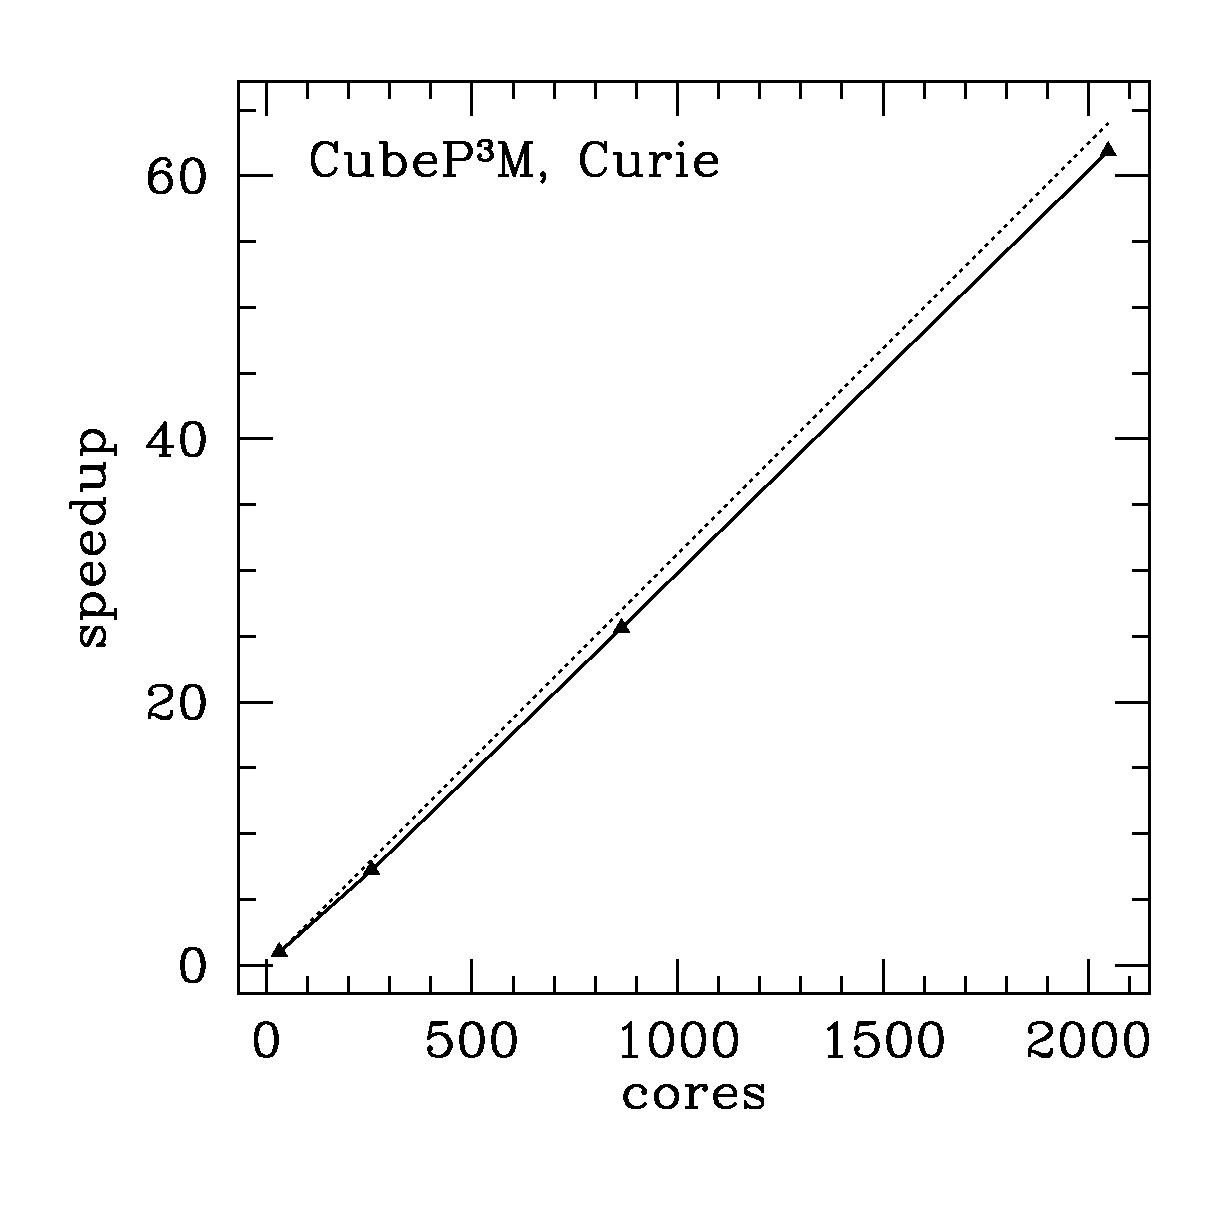
\includegraphics[width=3.2in]{graphs/scaling_cubep3m_curie.eps}
    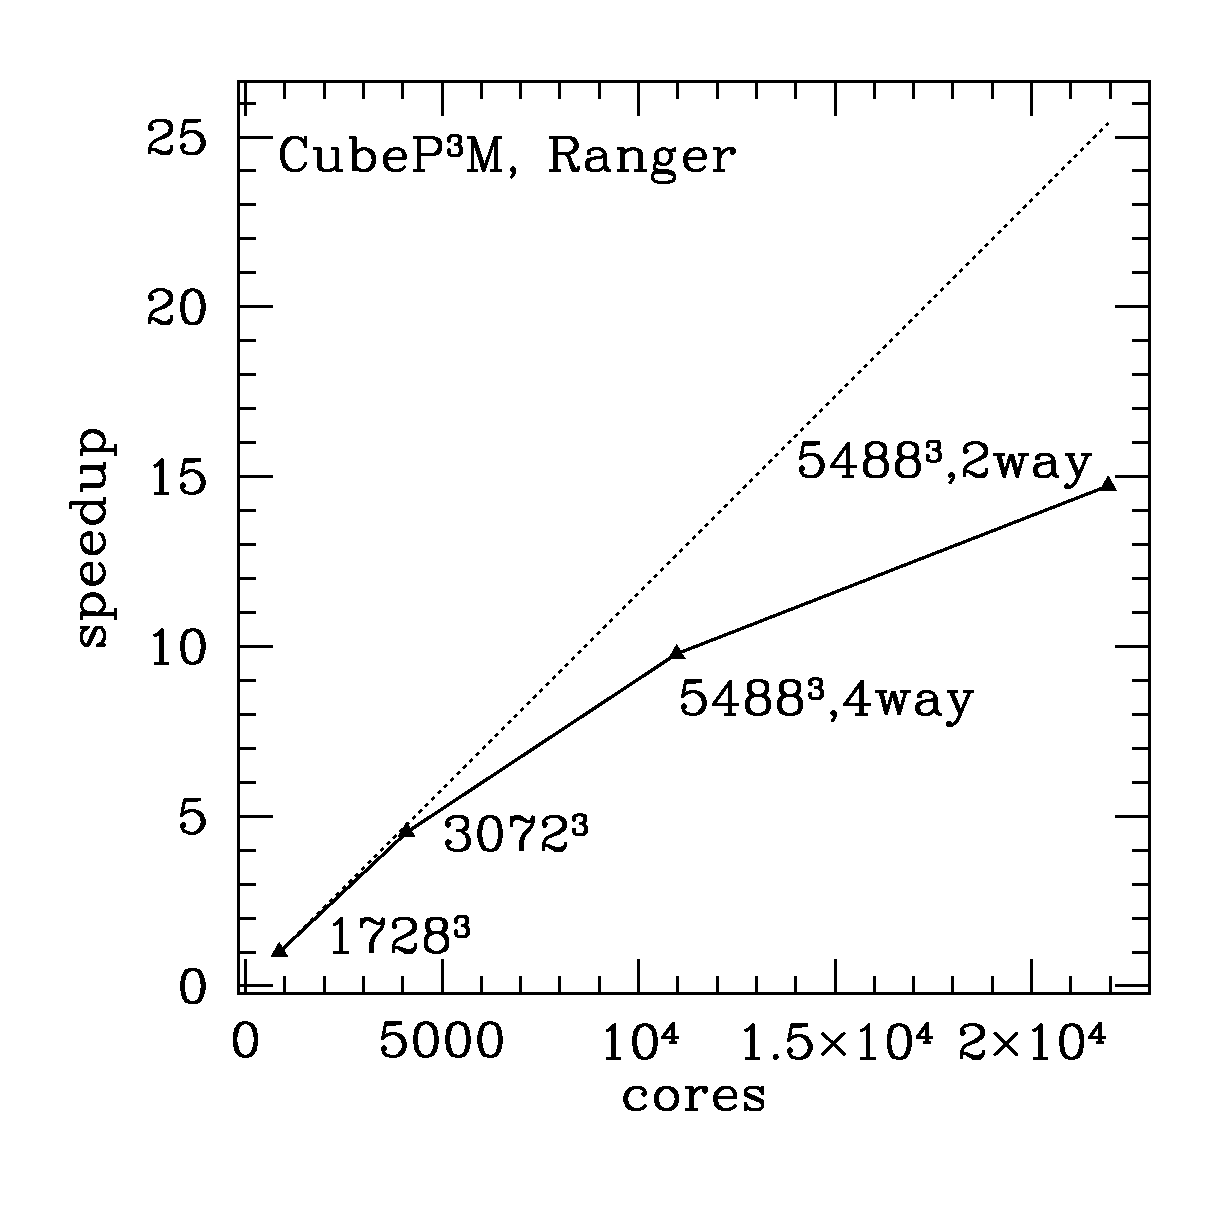
\includegraphics[width=3.2in]{graphs/scaling_cubep3m_new.eps}
%  \vskip -1.2cm 
%  \vskip -0.5cm 
  \caption{Scaling of {\small CUBEP3M} on Curie fat nodes (left) and 
    on Ranger TACC facility for very large number of cores (right). Plotted is the code speedup 
    ($N_{\rm particles}^3/t_{\rm wallclock}$) against core count, normalized by the smallest run 
    in each case. Dashed line indicates the ideal weak 
    scaling. The data are listed in Table \ref{summary_scaling_table}.
    \label{scaling}
% \vskip -0.9cm 
}
\end{center}
\end{figure*}

\begin{table*}%[ht]
  \vskip -0.5cm 
  \begin{center}
\caption{Scaling of {\small CUBEP3M} on Curie. Speedup is 
scaled to the smallest run.}
\label{summary_scaling_table}
\begin{tabular}{@{}|llllll|}
\hline
number of cores & speedup & ideal speedup & absolute timing (min) & 
$N_{\rm particles}$& box size ($h^{-1}$Mpc)
\\[2mm]\hline
%\hline
32  &  1.00 & - &3.2 & $256^3$ & 256\\
256  & 7.21 & 8 &3.55 & $512^3$  & 512\\
864  & 25.63 & 27 &4.8 & $864^3$  & 864\\
2048  & 61.87 & 64 &26.48 & $2048^3$ & 2048 \\
\hline
\end{tabular}
\caption{Scaling of  {\small CUBEP3M} on Ranger. Speedup is scaled to the smallest run.}
\label{summary_scaling_table2}
\begin{tabular}{@{}|llllll|}
\hline
number of cores & speedup & ideal speedup & absolute timing (min) & 
$N_{\rm particles}$& box size ($h^{-1}$Mpc)
\\[2mm]\hline
%\hline
864    & 1.00  & -    &258   & $1728^3$  & 6.3\\
4096   & 4.53  & 4.74 &320   & $3072^3$  & 11.4\\
10976  & 9.78  & 12.7 &845   & $5488^3$  & 20\\
21952  & 14.73 & 25.4 &561   & $5488^3$  & 20 \\
\hline
\end{tabular}
\end{center}
  \vskip -0.7cm 
\end{table*}

%the Ranger system at the Texas Supercomputing
%Center (in top 20 in the world) which is a SunBlade x6420 
%with AMD x86\_64 Opteron Quad Core 2300 MHz (9.2 GFlops)
% ``Barcelona'' processors and Infiniband networking. It has 
%a total of 62976 computing cores and 125952 GB of total 
%memory. Its nodes consist of 4 Quad Core processors and 32 GB 
%of shared RAM. For efficiency reasons (local memory access) we 
%typically use smaller MPI 'nodes' consisting of one Quad Core 
%processor and 8 GB of RAM. 

The parallel algorithm of {\small CUBEP3M} is designed for `weak' 
scaling, i.e. if the number of cores and the problem size 
increase in proportion to each other, then for ideal scaling the 
wall-clock time should remain the same. This is to be in contrasted with `strong' 
scaling codes, whereby the same problem solved on more cores should take 
proportionately less wall-clock time. This weak scaling requirement 
is dictated by the problems we are typically investigating (very 
large and computationally-intensive) and our goals, which are to 
address such large problems in the most efficient way, rather than 
for the least wall-clock time. Furthermore, we recall that there is no explicit 
load balancing feature, thus the code is maximally efficient when the sub-domains
contain roughly an  number of particles. This is true for most
cosmological-size volumes that do not resolve too deep in the non-linear regime, 
but not for e.g. simulations of a single highly-resolved galaxy. 

Because of the volumetric decomposition, the total number of {\small MPI} processes needs
to be a perfect cube. Also, for maximal resource usage, the number of tiles per node 
should be a multiple of the number of available {\small CPU}s per {\small MPI} process,
such that no core sits idle in the threaded block.
Given the available freedom in the parallel configuration, as long as the load is balanced, it is generally good practice to maximize the number of {\small OPENMP} threads and minimize the number of {\small MPI} processes:
the information exchange between cores that are part of the same motherboard is generally much faster.
In addition, having fewer {\small MPI} processes reduces the total amount of buffer zones, 
freeing memory that can be used to increase the mesh resolution. 
As one probes deeper into the non-linear regime however, 
the formation of dense objects can cause memory problems in such configurations, and increasing 
the number of {\small MPI} processes helps to ensure memory locality,
especially in non-uniform memory access (NUMA) environments.


%Since the current Curie is using Intel Nehalem architecture, while 
%the thin Curie nodes will use the newer Westermere Intel architecture, 
%we also show the scaling of our code on the Westermere-based Lonestar 
%computer at the Texas Advanced Computing Centre 


 The intermediary version of the code -- {\small CUBEPM} --
was first  ported to the IBM Blue Gene/L platform, and achieved 
weak-scaling up to 4096 processes (over a billion particles), with the N-body calculation only incurring a 10 per cent overhead 
at runtime (compared to 8 processes) for a balanced workload {\bf (How do we cite Hugh's work on blue gene?)}.  In order to 
accommodate the limited amount of memory available per processing core on the 
Blue Gene/L platform machines, it was necessary to perform the long range {\small MPI FFT}
with a volumetric decomposition \citep{3DFFT}.
Slab decomposition would have required a volume too large to fit in system 
memory given the constraints in the simulation geometry. 

 
The scaling of {\small CUBEP3M}  was first  tested with a dedicated series 
of simulations -- the CURIE simulation suite-- by increasing the size and number of cores on the `fat' 
(i.e. large-memory) nodes of the  Curie supercomputer at the Tr\`{e}s Grand Centre de Calcul (TGCC) in France. 
 For appropriate direct comparison,
all these simulations were performed using the same particle mass 
($M_{\rm particle}=1.07\times10^{11}M_\odot$) and force resolution 
(softening length 50 $h^{-1}$kpc). The box sizes used range from 256 $h^{-1}$Mpc
to 2048 $h^{-1}$Mpc, and the number of particles from $256^3$ to $2048^3$.
Simulations were run on 32 up to 2048 computing cores, also starting from 
redshift $z=100$, and evolving until $z=0$. Our results are shown in Fig. \ref{scaling} and in Table \ref{summary_scaling_table}, and present excellent scaling, within 
$\sim3$ per cent of ideal, at least for up to 2048 cores. 



We have also ran {\small CUBEP3M} on a much larger number of cores, 
from 8000 to up to 21,976, with $5488^3$-$6000^3$ (165 to 216 billion) 
particles on Ranger and on JUROPA at the J\"ulich Supercomputing Centre in Germany, 
which is an Intel Xeon X5570 
(Nehalem-EP) quad-core 2.93 GHz system, also interconnected with Infiniband.
Since it is not practical to perform dedicated scaling tests on such a large number of
computing cores, we instead list in Table \ref{summary_scaling_table2} 
the data directly extracted from production runs. We have found the 
code to scale within 1.5 per cent of ideal up to 4096 cores. 
For larger sizes ($\ge$10,976 cores), the scaling is less ideal,
due to increased communication 
costs, I/O overheads (a single timeslice of $5488^3$ particles is 3.6 TB)
and load balancing issues, but still within $\sim20$ per cent of ideal. 
These first three Ranger runs were performed 
with 4 {\small MPI} processes and 4 threads per Ranger node (`4way')\footnote{For these very large runs, 
we used a NUMA script {\it tacc\_affinity}, specially-provided by the technical staff, 
that bind the memory usage to local sockets, thus ensuring memory affinity. 
This becomes important because the memory sockets per node 
(32 GB RAM/node on Ranger) are actually not equal-access. Generally, the local 
memory of each processor has much shorter access time.}.

Furthermore, due to the increasing clustering of structures at those small 
scales, some of the cuboid sub-domains came to contain a number of particles
well above the 
average, thereby requiring more memory per {\small MPI} process
in order to run until the end. 
As a consequence,  throughout most of their late evolution, the 
largest two of these simulations were run with 4096 and 21,952 cores and 
with only 2 {\small MPI} processes and 8 threads per Ranger node (`2way'), which on 
Ranger allows using up to 16 GB of RAM per {\small MPI} process\footnote{In order to insure 
local memory affinity,  a second special NUMA control script, {\it tacc\_affinity\_2way}, 
was developed for us by the TACC technical staff and allowed to run more efficiently 
in this mode.}. Because each processor accesses memory that is not fully local, this configuration does affect the 
performance somewhat, as does the imperfect load balancing that arises in such situations.
This can be seen in the rightmost point of FIg. \ref{scaling} (right panel), where the scaling 42 per cent below the ideal.
We note that we still get $\sim1.5$ speedup
from doubling the core count, even given these issues. Overall the
code scaling performance is thus satisfactory even at extremely large number of cores.
 We expect the code to handle even larger problems efficiently, and is thus well suited to run on
  next generation Petascale systems. 

Finally, we note that several special fixes had to be developed by  the TACC 
and JUROPA technical staff in order for our largest runs to work properly.
In particular, we encountered unexpected problems from software libraries such as 
{\small MPICH} and {\small FFTW} when applied to calculations of such 
unprecedented size. 

{\bf (We should also compare the memory usage to other codes like Gadget. Ilian mentioned Gadget uses 90 Bytes per particle. Is cubep3m really using 130 Bytes per particle? Check with mem\_usage.)}

\section{Accuracy}
\label{sec:accuracy}
 
One of the most reliable way to assess the simulation's accuracy at evolving particles
is to measure the density power spectrum at late time, and compare to non-linear prediction. 
For an over-density field $\delta({\bf \it x})$, the power spectrum is extracted from the two point function in Fourier space as:
\begin{eqnarray}
\langle | \delta ({\bf \it k}) \delta ({\bf \it k'}) | \rangle = (2\pi)^{3}P(k)\delta_{D}({\bf \it k'} - {\bf \it k})
\label{eq:power}
\end{eqnarray}
where the angle bracket corresponds to an ensemble (or volume) average.
We plot in Fig. \ref{fig:power_highres} the dimensionless power spectrum in a RANGER4000 simulation and
observe that the agreement with the non-linear prediction of \cite{Lewis:1999bs} is at the per cent level over a large dynamical range.
The drop of power at high-$k$ is caused by the finite resolution, and the fluctuations at low-$k$ are caused by the white noise imposed in the initial conditions. {\b (I should add a vertical line at the k of the coarse mesh for visualization purposes.)}

\begin{figure*}%[ht]
  \begin{center}
    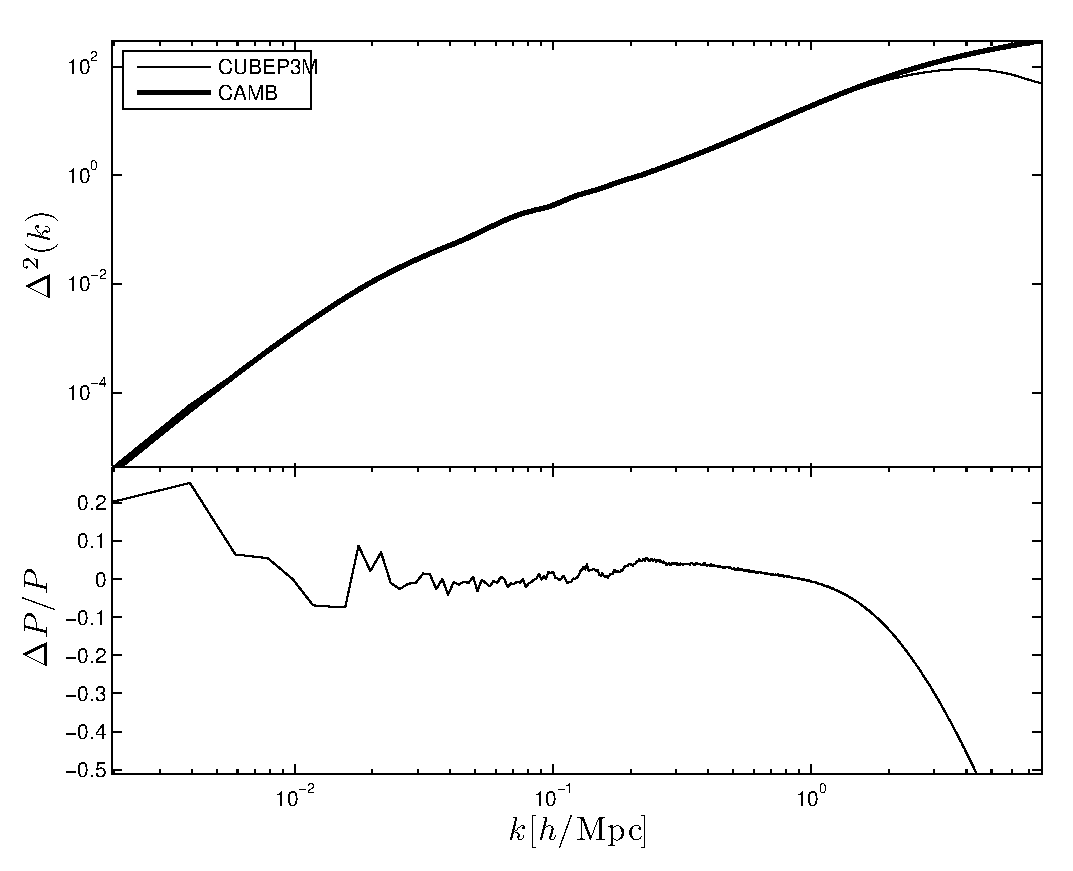
\includegraphics[width=5.2in]{graphs/power_highres.eps}
  \caption{Dark matter power spectrum, measured at $z=0$ in a RANGER4000 simulation,
  compared to the non-linear predictions of {\small CAMB}.
    \label{fig:power_highres}}
\end{center}
\end{figure*}

The actual force of gravity in the P$^3$M algorithm,
as felt by a single particle, is presented in Fig. \ref{fig:den_force_ppext0}.
This shows the force versus distance -- in fine cell units -- a calculation that was performed from a CITA256 realization in two steps: 
1- we compute the force on each particle in a given time step.
2- we remove a selected particle, compute the force again on all particles, and record on file the 
force difference (before  and after the removal) as a function of the distance to the `hole'.

Particles in the same fine cell as the hole follow the exact $1/r^{2}$ curve. The scatter at 
  distances of the order of the fine grid is caused by the NGP interpolation scheme:
  particles in adjacent fine cells can be actually very close, as seen in the upper left region of this plot,
  but still feel the mesh force at grid cell distances,
  creating up to an order of magnitude loss.
As the separation approaches a tenth of the full box size or so, the force on the coarse mesh deviates
from Newton's law in order to preserve periodic boundary conditions. 
This feature, however, can be turned off at compilation time.


Fig. \ref{fig:den_force_fracErr} shows the fractional error on the force along the radial and tangential directions.
It is larger than in {\small PMFAST} at grid scales, largely due to the fact that the fine mesh force is performed with an NGP interpolation scheme -- as opposed to CIC -- which shows a larger scatter about the theoretical value. 
As discuss in the next section, to minimize this effect, we apply a random offset to all the particles,
such that this undesired scatter is averaged out over a few time steps.



\begin{figure}%[ht]
  \begin{center}
    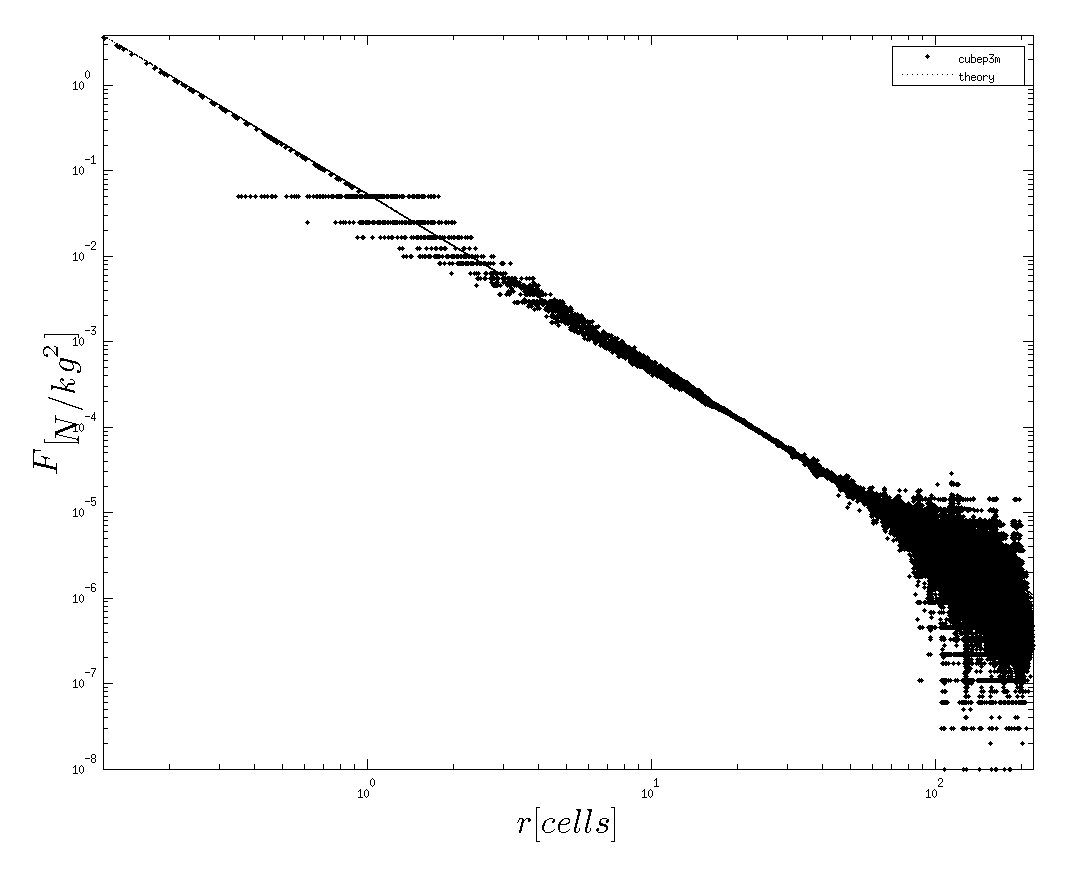
\includegraphics[width=3.2in]{graphs/densityForce_ppext=0.eps}
  \caption{Gravity force in of the P$^3$M algorithm, versus distance in fine mesh cell units, compared with the exact $1/r^{2}$ law.
    This particular calculation was obtained in a CITA256 realization with  a box size of $500 h^{-1}\mbox{Mpc}$,
    in a single time step. In a full simulation run, the scatter averages over many time steps, thanks to the inclusion of a random offset that is imposed on each particle. 
    \label{fig:den_force_ppext0}}
\end{center}
\end{figure}

\begin{figure}%[ht]
  \begin{center}
    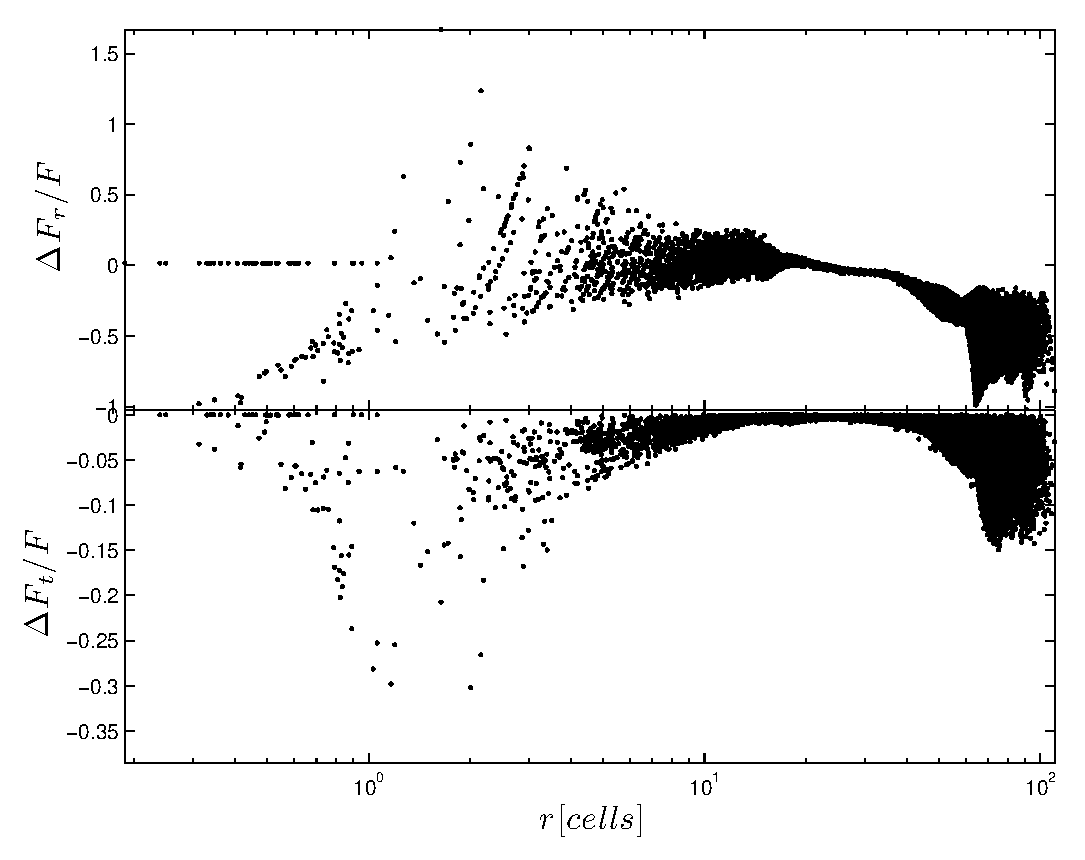
\includegraphics[width=3.2in]{graphs/densityForce_fracErr.eps}
  \caption{Fractional error on the force in of the P$^3$M algorithm, in the radial (top) and tangential (bottom) directions.
  This scatter is significantly reduced with the random offset, as discussed in section \ref{sec:systematics}.
    \label{fig:den_force_fracErr}}
\end{center}
\end{figure}


\section{Systematics}
\label{sec:systematics}

\subsection{Mesh force at grid distances}

The biggest problem with the straightforward pp force calculation is that the results 
are anisotropic and depend on the location of the fine mesh with respect 
to the particles. As an example, consider two particles on either side of a grid 
cell boundary, experiencing their mutual gravity attraction via the fine mesh force with a discretized 1-grid cell separation.
 If, instead, the mesh was shifted such that they were
within the same cell, they would experience the much larger pp force. 
This effect is especially pronounced at the early stages of the simulation where
the density is more homogeneous, and leads to mesh artefacts appearing
in the density field. In order to minimize this systematic effect, 
we randomly shift the particle distribution relative to the mesh by a small
amount -- up to 2 fine grid cells in magnitude -- in each
dimension and at each time step.  This adds negligible computational
overhead as it is applied during the particle position update,
and suppresses the mesh behaviour that otherwise grows over multiple time steps.
It is possible to shift back the particles at the end of each time steps,
which prevents a random drift of the whole population, a necessary step 
if one needs to correlate the initial and final positions of the particles for instance,
or for hybrid dark matter -- MHD simulations.
 
We ensure that, on average, this solution balances out the mesh feature,
by tuning the force kernels such as to provide  force as evenly balanced as possible at grid cell distances
and at the cutoff length ($r_{c}=16$ fine cells).
These adjustments are performed from the pairwise force test described in section \ref{sec:accuracy}.
We note that this is one of the driving argument to extend the pp force outside the fine mesh cell,
since the scattering of the NGP force about the actual $1/r^{2}$ law drops rapidly as the distance increases.
As discussed in section \ref{subsec:extendedpp}, this gain in accuracy comes at a price,
a choice that  must be carefully balanced.

We present in Fig. \ref{fig:disp_mesh} the dramatic impact of removing the random offset in the code.
The power spectrum is completely wrong, due to the large scatter in the force from the fine mesh.
In this scatter is not averaged over, the error directly adds up at each time step. {\small PMFAST}
did not have this problem since it used CIC interpolation on both meshes.  
This test was performed with CITA256 simulations of very large box size,
which should in principle agree with linear predictions up to the resolution.
The output redshifts are very early, and the upper most curve ($z=10$) was obtained after
about 60 time steps.
We see that deviations are enormous when the random offset is turned off.

\begin{figure}%[ht]
  \begin{center}
    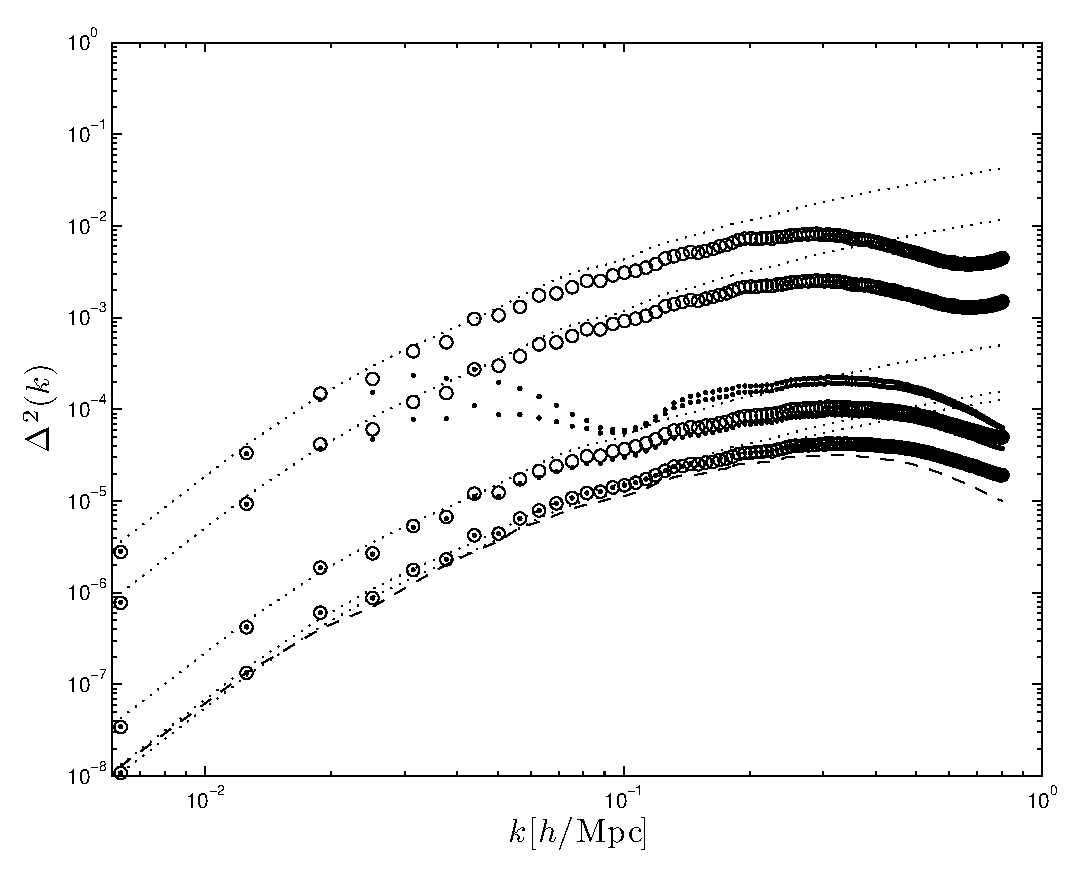
\includegraphics[width=3.2in]{graphs/power_w_wo_disp_mesh.eps}
  \caption{Dark matter power spectrum, measured at $z=180$, $100$, $20$ and $10$, in a series of CITA256 realizations that are 1000 Mpc/$h$ per side. The dashed line represent the initial condition power spectrum, the dotted lines are the linear predictions, and  the open circles the standard P$^3$M configuration. 
  The dots were obtained by simply removing the random particle offset that is usually applied at each time step. \label{fig:disp_mesh}}
\end{center}
\end{figure}

{\bf (Show how averaging over $~sim10$ time steps reduces the scatter.)}


\subsection{Constraining redshift jumps}

At early stages of the simulation, the density fields is rather homogenous, causing the force of gravity to be
rather weak everywhere. In that case, the size of the redshift jumps is controlled by a limit in the cosmological expansion.
If the expansion jump is too large, the size of the residual errors can become significant, and one can observe, for instance,
a growth of structure that does not match the predictions of  linear theory even at the largest scales.
One therefore needs to choose a maximum step size. In {\small CUBEP3M}, this is controlled by $r_{max}$, which is the fractional step size,
$\mbox{d}a/(a + \mbox{d}a)$ and is set to $0.05$ by default.  Generally, a simulation should start at a redshift high enough that
the initial dimensionless power spectrum is well under unity at all scales. This ensures that the Zel'dovich approximation
 holds at the per cent level at least. A drop of accuracy can occur if one starts the simulation too early, where
 truncation error will be significant at the early time steps.


It is possible to reduce this effect, and thereby improve significantly 
the accuracy of the code, by modifying the value of $r_{max}$, at the cost of increasing the total number of time steps.
Fig. \ref{fig:ra_max} shows a comparison of late time power spectra of a series of CITA256 realizations that originate from the same initial conditions, 
and used the same random seeds to control the fine mesh shifts (mentioned above): only the value of $r_{max}$ was modified between each run. 
We observe that the impact is mostly located in the non-linear regime, where decreasing the time step to 0.006 
allows the simulation to recover about 30 per cent of dimensionless power at the turn over scale, in this simulation configuration.
This gain is greatly affected by the choice of initial redshift, the resolution, and the box size, and ideally one would make
test runs in order to optimize a given configuration.  
As expected, the {\small CPU} resources required to run these simulations increase rapidly as $r_{max}$ decreases, as seen in Table \ref{table:ra_max}. 
In this test case, reducing further at 0.001 shows only a mild improvement in accuracy, but the increase in time is more than a factor of four.
We should mention that with a proper use of the non-Gaussian initial conditions, it is possible to start the simulations at much later redshifts, where the time step sizes are dominated by a stronger mesh force.
 

\begin{figure}%[ht]
  \begin{center}
    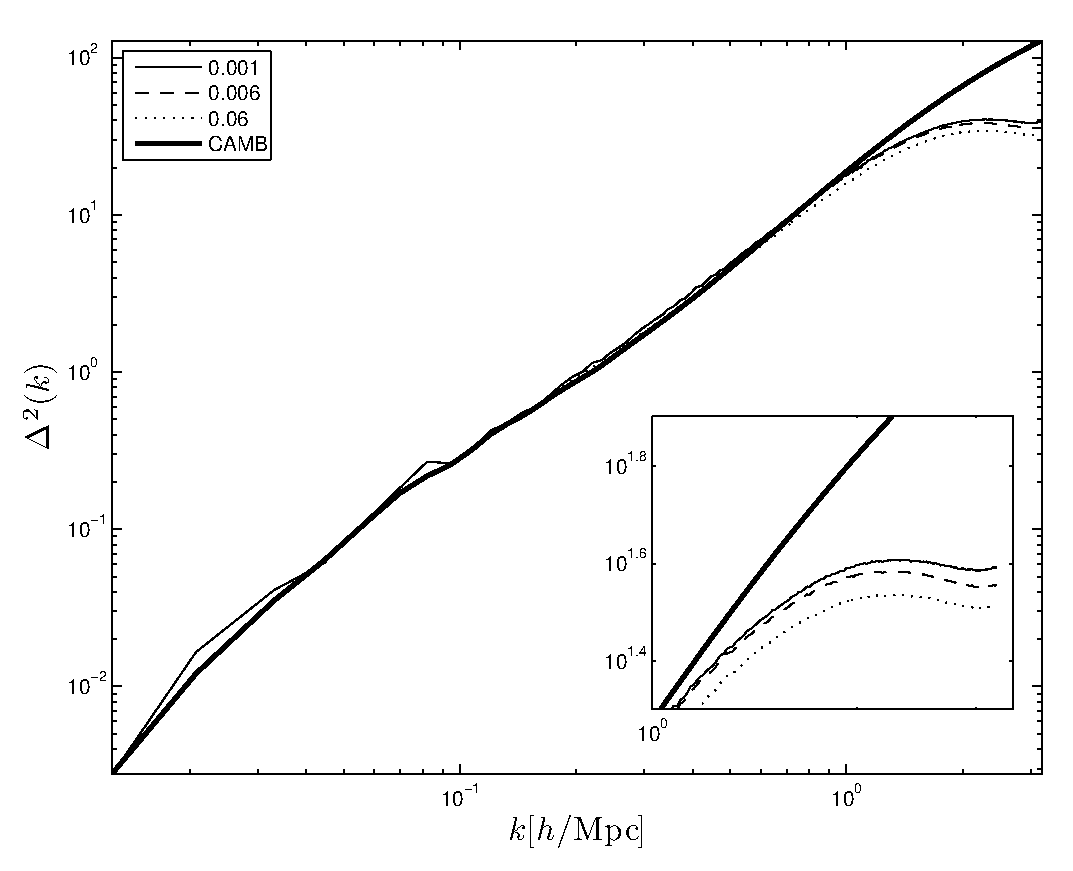
\includegraphics[width=3.2in]{graphs/power_ra_max.eps}
  \caption{Dark matter power spectrum, measured at $z=0$ in a series of CITA256 realizations. 
 The starting redshift ofwas raised to $z=200$ to enhance the systematic effect. The different curves show different values of $r_{max}$. 
  The resources required to run these simulations increase rapidly as $r_{max}$ decreases, as seen in Table \ref{table:ra_max}.    \label{fig:ra_max}}
\end{center}
\end{figure}

\begin{table}
\begin{center}
\caption{Scaling in {\small CPU} resources as a function of the value of $r_{max}$. The tests were performed 
on the CITA Sunnyvale cluster, and general trends could vary slightly on other machines.}
\begin{tabular}{|l|c|c|}
\hline 
$r_{max}$         & time (h)   \\                 
\hline
 $0.1$ & 1.46 \\
 $0.06$ & 1.48\\
 $0.01$ & 1.67 \\
 $0.006$ & 1.91\\
 $0.003$ & 2.83 \\
 $0.002$ & 4.13\\
 $0.001$ & 8.15\\
\hline
\end{tabular}
\label{table:ra_max}
\end{center}
\end{table}


{\bf (Any other systematics effects we want to discuss here?)}

 



\section{Runtime Halo Finder}
\label{sec:halo}

%Spherical overdensities, search algorithm, 
%provided halo information, halo bias, comparison to PS and ST.
%{\bf (Ilian, You can lead the way here...)}

We have implemented a halo finding procedure, which we have developed 
based on the spherical overdensity (SO) approach \citep{1994MNRAS.271..676L}.
In the interest of speed and efficiency the halo catalogues are constructed 
on-the-fly at a pre-determined list of redshifts. The halo finding is 
massively-parallel and threaded based on the main {\small CUBEP3M} data structures 
discussed in section \ref{sec:structure}. The code first builds the 
fine-mesh density for each sub-domain using CIC or NGP interpolation. It then 
proceeds to search for and record all local density maxima above certain
threshold (typically set to 100 above mean density) within the local 
sub-domain's physical volume (excluding the sub-domain buffer zones). It then 
uses parabolic interpolation on the density field to determine more precisely
the location of the maximum within the densest cell, and records the peak 
position and value. The halo centre determined this way agrees closely with 
the centre-of-mass of the halo particles discussed below.  

Once the list of peak positions is generated, they are sorted from the highest 
to the lowest density value. Then each of the halo candidates is inspected 
independently, starting with the highest peak. The grid mass is accumulated 
in spherical shells of fine grid cells surrounding the maximum, until the 
mean density within the halo drops below a pre-defined overdensity cutoff 
(usually set to 178 in units of the mean, in accordance to the top-hat 
collapse model). As we accumulate mass we remove it from the mesh, so that no 
mass element is double-counted. This method is thus inappropriate for finding 
sub-halos as within this framework those are naturally incorporated in their 
host halos. Because the halos are found on a grid of finite-size cells, it is 
possible, especially for the low-mass halos, to overshoot the target overdensity.
When this occurs we use an analytical halo density profile to correct the 
halo mass and radius to the values corresponding to the target overdensity. 
This analytical density profile is given by Truncated Isothermal Sphere (TIS) 
profile \citep{1999MNRAS.307..203S,2001MNRAS.325..468I} for overdensities below 
$\sim130$, and $1/r^2$ for lower overdensities. The density profile has a
similar outer slope (the relevant one here) to the Navarro, Frenk and White 
\citep[NFW][]{1997ApJ...490..493N} profile, but extends to lower overdensities
and matches well the virialization shock position given by the Bertschinger 
self-similar collapse solution \citep{1985ApJS...58...39B}.

Once the correct halo mass, radius and position are determined, we find all 
particles which are within the halo radius. Their positions and velocities are
used to calculate the halo centre-of-mass, bulk velocity, internal velocity 
dispersion and the three angular momentum components, all of which are then 
included in the final halo catalogues. We also calculate the total mass of
all particles within the halo radius, also listed in the halo data. This mass
is very close, but  typically slightly lower, than the halo mass calculated 
based on the gridded density field. The particle centre-of-mass corresponds 
very well to the halo centre found based on the gridded mass distribution. 

%Compared to Tinker
%44% low for 50 particles
%22% low for 400 particles
%12% low for 1000 particles

\begin{figure}%[ht]
%  \vskip -0.5cm 
  \begin{center}
    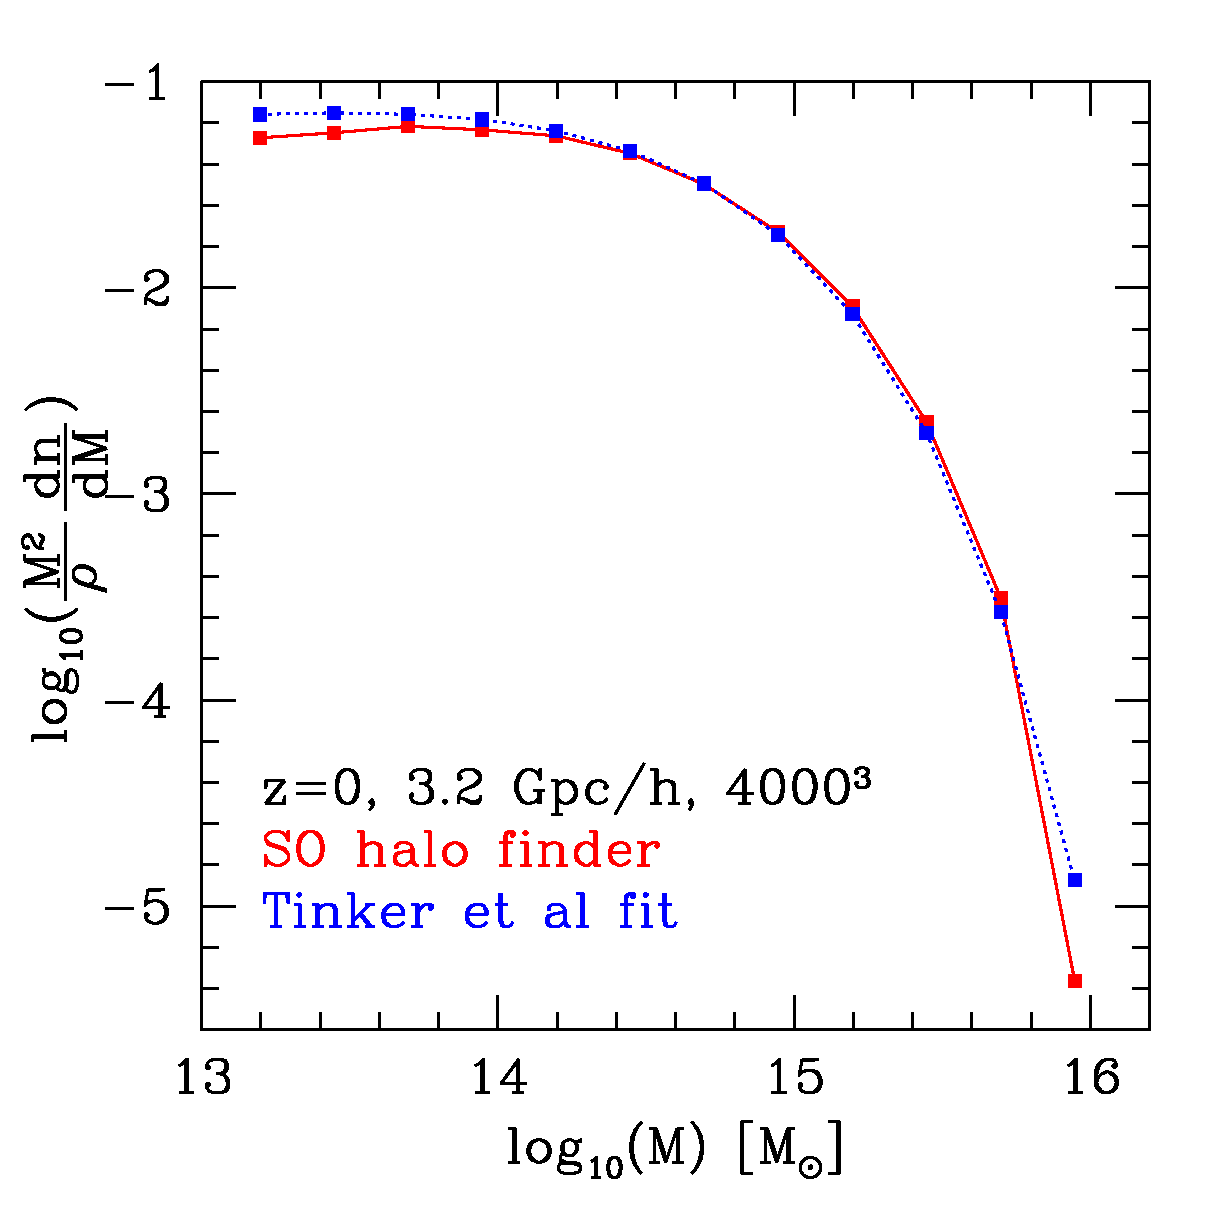
\includegraphics[width=3.2in]{graphs/mf_z0_Tinker.eps}
  \end{center}
  \caption{Simulated halo multiplicity function, 
    $\frac{M^2}{\bar{\rho}}\frac{dn}{dM}$ based on a
    RANGER4000 simulation with $3.2\,h^{-1} \mbox{Gpc}$ box and $4000^3$ 
    particles (solid, red in the online version). For reference we also show a widely-used 
    precise fit by \citet{2008ApJ...688..709T} (blue, dashed). 
    \label{mf}}
\end{figure}

A sample halo mass function produced based on our inlined SO halo finder 
at redshift $z=0$ from a RANGER4000 simulation is shown in Fig. \ref{mf}. We compare our result to the 
precise fit presented recently by \citet{2008ApJ...688..709T}. Unlike most
other widely-used fits like the one by \citet{2002MNRAS.329...61S}, which are based on friends-of-friends (FOF)
halo finders, the \citet{2008ApJ...688..709T} fit is based on the
SO search algorithm, whose masses are systematically different 
from the FOF masses \citep[e.g.][]{2007MNRAS.374....2R,2008ApJ...688..709T}, 
making this fit a better base for comparison here. Results show excellent
agreement, within $\sim10$ per cent for all halos with masses corresponding to
1000 particles or more. Lower-mass halos are somewhat under-counted compared
to the \citet{2008ApJ...688..709T} fit, by $\sim20$ per cent for 400 particles and 
by $\sim40$ per cent for 50 particles. This is due to the grid-based nature of our
SO halo finder, which misses some of the low-mass halos. It was shown, however, that using more sophisticated
halo finders (available through post-processing due to their heavier memory
footprint) allows to recover the expected mass function.

A second test of the accuracy of the halo finder algorithm is to extract the halo power spectrum $P_{h}(k)$ and compare the halo bias
with theoretical predictions. The halo bias is defined as $b(k) = \sqrt{P(k)/P_{h}(k)}$ and is shown in Fig. \ref{fig:halo}.
{\bf Expand here, describe, match with theory, etc...}
\begin{figure}%[ht]
%  \vskip -0.5cm 
  \begin{center}
    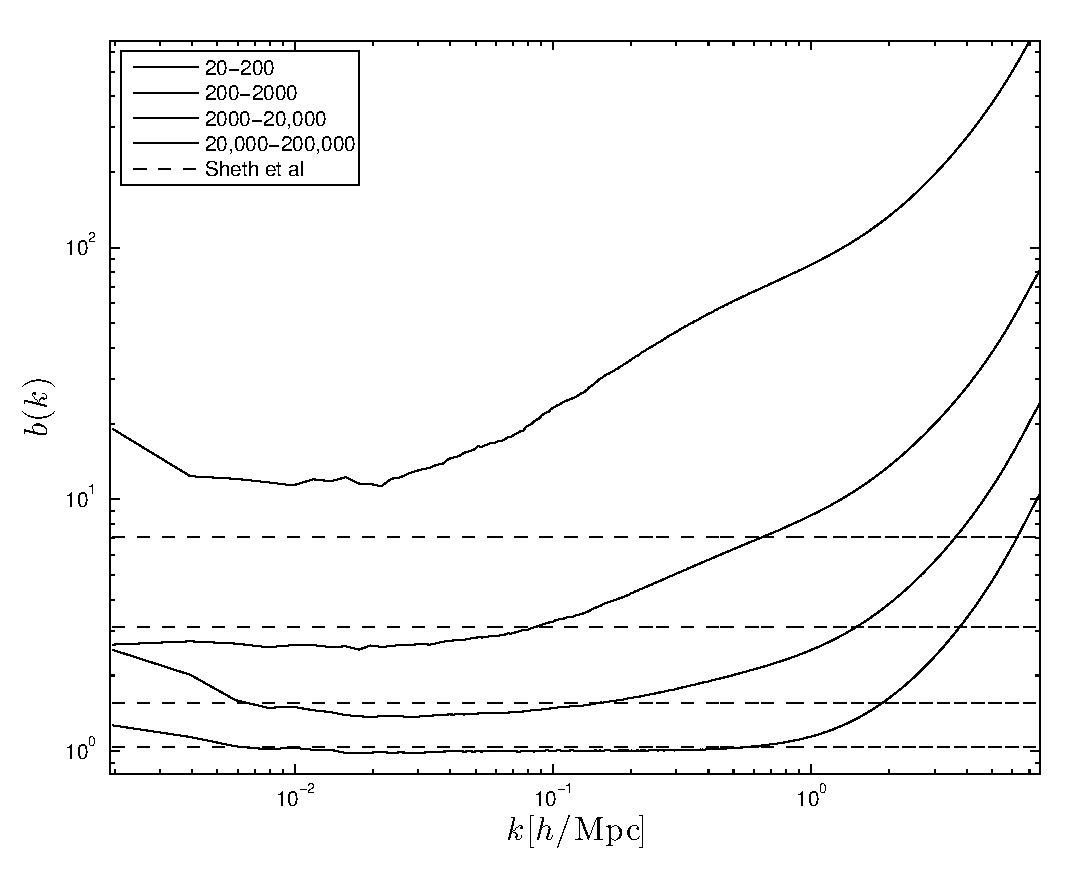
\includegraphics[width=3.2in]{graphs/bias.eps}
  \end{center}
  \caption{Halo bias, measured at $z=0$ from a RANGER4000 simulation with a side length of $3.2 h^{-1}$Gpc.
  Bottom to top curves correspond to haloes of different masses, from light to massive. The four bins are decades
  of halo masses; the first contains haloes made of 20-200 particles, the second of 200-2,000 and so on.
    \label{fig:halo}}
\end{figure}


%{\bf Show some examples and comparisions to analytical fits and other halo finders.}

\section{Beyond the standard configuration}
\label{sec:extensions}

The preceding descriptions and discussions apply to the standard configuration of the code, 
as described at the beginning of section \ref{sec:structure}. A few extensions have been recently developed
in order to enlarge the range of applications of {\small CUBEP3M}, and this section briefly 
describe the most important improvements.


%%\subsection{Generalization of the dark energy equation of state}
%\label{subsec:runningomegal}
%
%The cosmic expansion is obtained from a third order Taylor expansion in the scale factor of Friedmann's equation,
%and has now the flexibility to accomodate a running equation of state of the form $\omega(a) = \omega_0 + a\omega_1$,
%which is the standard parameterization adopted by the Dark Energy Task Force \citep{2006astro.ph..9591A}.
%The code also currently supports expansion under a modified Chaplygin gas cosmology\cite{Chaplygin}. 
%{\bf Is this worth mentioning at all?}

%{}
 

\section{Conclusion}

This paper describes {\small CUBEP3M}, a public and  massively parallel P$^3$M N-body code that inherits from {\small PMFAST} 
 and that now scales well to 20,000 cores, pushing the limits of the cosmological problem size one can handle.
We summarize the code structure, review the double-mesh Poisson solver algorithm, and present scaling and systematic tests
that have been performed. We also describe various utilities and extensions that come with the public release, 
including a run time halo finder, an extended pp force calculation and a non-Gaussian initial condition generator.
{\small CUBEP3M} is one of the most competitive N-body code that is publicly available for cosmologists and astrophysicists,
it has already been used  for a large number of scientific applications, and it is our hope that the current documentation will 
help the community in interpreting its outcome.
The code is publicly available on github.com under {\tt cubep3m}, and extra documentation about the structure, 
compiling and running strategy is can be found on the CITA wiki page\footnote{\tt www.wiki.cita.utoronto.ca/mediawiki/index.php/CubePM}.

\section*{Acknowledgements}

The CITA simulations were run on the Sunnyvale cluster at CITA.
ITI was supported by The Southeast Physics
Network (SEPNet) and the Science and Technology Facilities Council
grants ST/F002858/1 and ST/I000976/1. 
Computations for the SciNet1024 runs were performed on the GPC supercomputer at the SciNet HPC Consortium. SciNet is funded by: the Canada Foundation for Innovation under the auspices of Compute Canada; the Government of Ontario; Ontario Research Fund - Research Excellence; and the University of Toronto. 
The authors acknowledge the
TeraGrid and the Texas Advanced Computing Center (TACC) at The
University of Texas at Austin (URL: http://www.tacc.utexas.edu) for
providing HPC and visualization resources that have contributed to the
research results reported within this paper. ITI also acknowledges the Partnership for Advanced
Computing in Europe (PRACE) grant 2010PA0442 which supported the code
scaling studies. UEP and JDE are supported by the NSERC of Canada.
%{\bf ( Hugh, Vincent, JD, any financial acknowledgements to add here?)}


%\input{Appendix}
\bibliographystyle{mn2e}
\bibliography{mybib3_new}{}
%\bibliographystyle{amsplain}

\bsp

\label{lastpage}


\end{document}
